% CVPR 2027 submission — GenAU.
% Ported from the ICLR 2027 version (this same directory, before the rename) and,
% for the two-column scaffolding, from the WACV 2027 version in ../GenAU.
% See PORTING_NOTES.md.
%
% Build: pdflatex main -> bibtex main -> pdflatex main -> pdflatex main -> pdflatex main
% (the third pass after bibtex is needed for the pagebackref lists to settle)
%
% NOTE ON THE TEMPLATE YEAR: there is no CVPR 2027 author kit yet (the newest
% official release is CVPR2026-v1(latex); github.com/cvpr-org/author-kit main was
% last updated 2026-05-28 and still says 2026). cvpr.sty is byte-identical to that
% official file — every user-visible year comes from \confYear below, which is the
% only thing that has changed between kit years. Re-check when the 2027 kit drops.

\documentclass[10pt,twocolumn,letterpaper]{article}

%%%%%%%%% PAPER TYPE  - PLEASE UPDATE FOR FINAL VERSION
\usepackage[review]{cvpr}      % To produce the REVIEW version
% \usepackage{cvpr}              % To produce the CAMERA-READY version
% \usepackage[pagenumbers]{cvpr} % To force page numbers, e.g. for an arXiv version

% Import additional packages in the preamble file, before hyperref
%
% CVPR preamble.
%
% cvpr.sty already provides: times, xspace, xcolor[dvipsnames], graphicx,
% amsmath, amssymb, booktabs, natbib[numbers,sort&compress], silence, etoolbox,
% caption, subcaption, url and enumitem -- and it loads cleveref itself via
% \AtEndPreamble (i.e. strictly after hyperref), so none of those may be loaded
% here. (This is the same package set wacv.sty supplied; the ICLR port had to
% declare them all by hand because iclr2027_conference.sty supplied only
% fancyhdr + natbib.)
%
% Disable PDF object-stream compression: the large architecture figure this
% was added for (the former imgs/GenAU_Arch_final.pdf) otherwise overflowed pdfTeX's
% object-stream buffer ("TeX capacity exceeded [PDF object stream buffer]").
\ifdefined\pdfobjcompresslevel \pdfobjcompresslevel=0 \fi

% --- required by this paper and NOT provided by cvpr.sty ---
\usepackage{multirow}   % \multirow in the result/ablation tables
\usepackage{colortbl}   % \rowcolor{gray!20} (the "table" feature of xcolor)
\usepackage{tabularx}   % column-width ablation table (Table 2)
\usepackage{tikz}       % motivation radar chart (Fig. 1)
\usepackage{microtype}  % char protrusion + font expansion: tighter lines, fewer runts

% --- compact (but standard) float spacing to help fit the page limit ---
\setlength{\textfloatsep}{10pt plus 2pt minus 2pt}      % top/bottom single-col floats
\setlength{\intextsep}{10pt plus 2pt minus 2pt}         % [h] floats
\setlength{\dbltextfloatsep}{12pt plus 2pt minus 2pt}   % full-width figure*/table*

% --- ablation-table deltas to the default row: fixed-width box keeps the numbers aligned
\newcommand{\abd}[2]{\makebox[1.9em][l]{\textsubscript{\textcolor{#1}{#2}}}}
\newcommand{\abup}[1]{\abd{ForestGreen}{$+$#1}}
\newcommand{\abdn}[1]{\abd{BrickRed}{$-$#1}}
\newcommand{\abeq}{\abd{gray}{$\pm$0.0}}
\newcommand{\abno}{\abd{black}{}}

% --- inline annotations
\newcommand{\red}[1]{{\color{red}#1}}
\newcommand{\todo}[1]{{\color{red}#1}}
\newcommand{\TODO}[1]{\textbf{\color{red}[TODO: #1]}}
% --- disable by uncommenting
% \renewcommand{\TODO}[1]{}
% \renewcommand{\todo}[1]{#1}


% hyperref with pagebackref eases the reviewers' job. cvpr.sty loads cleveref
% itself (\AtEndPreamble, i.e. strictly after hyperref), so do NOT load it here.
\definecolor{cvprblue}{rgb}{0.21,0.49,0.74}
\usepackage[pagebackref,breaklinks,colorlinks,allcolors=cvprblue]{hyperref}

%%%%%%%%% PAPER ID  - PLEASE UPDATE
\def\paperID{*****} % *** Enter the Paper ID here
\def\confName{CVPR}
\def\confYear{2027}

%%%%%%%%% TITLE - PLEASE UPDATE
% "Language-Grounded" dropped: the learned-query control does not support it (Appendix, anchor seeds).
% Alternatives:
%   GenAU: A Generalist Vision-Language Model for Industrial Anomaly Understanding
%   GenAU: Unifying Anomaly Detection, Segmentation, and Explanation in One Vision-Language Model
\title{GenAU: One Vision-Language Model to Detect, Segment, Classify, and Explain Industrial Anomalies}

%%%%%%%%% AUTHORS - PLEASE UPDATE
% CVPR review submissions are double-blind. With \usepackage[review]{cvpr} the
% style prints "Anonymous CVPR submission / Paper ID \paperID" instead of this
% block, so it only matters for the camera-ready.
\author{First Author\\
Institution1\\
Institution1 address\\
{\tt\small firstauthor@i1.org}
% For a paper whose authors are all at the same institution,
% omit the following lines up until the closing ``}''.
% Additional authors and addresses can be added with ``\and'',
% just like the second author.
% To save space, use either the email address or home page, not both
\and
Second Author\\
Institution2\\
First line of institution2 address\\
{\tt\small secondauthor@i2.org}
}

\begin{document}
\maketitle

% \begin{abstract}
% Industrial anomaly detection is critical for product quality assurance and process reliability, yet practical inspection requires more than determining whether an image is normal or anomalous. A useful system should also localize defective regions, recognize different defect types, and provide interpretable defect analysis and diagnosis. Existing CLIP-based methods have shown strong performance in binary anomaly detection and segmentation, yet most of them remain limited to binary discrimination and offer only weak support for fine-grained defect understanding. Meanwhile, recent autoregressive vision-language models (VLMs) provide powerful multimodal reasoning and defect description capabilities, but existing VLM-based approaches are limited to text outputs and cannot directly produce pixel-level segmentation masks. As a result, a generalist model that unifies detection, segmentation, multi-type anomaly recognition, and defect analysis remains missing. 
% We present GenAU, a \textbf{G}eneralist vision-language framework for industrial \textbf{A}nomaly \textbf{U}nderstanding that unifies anomaly detection, anomaly segmentation, multi-type anomaly detection, and defect analysis within a single model. Specifically, we extend an instruction-following VLM with two segmentation tokens, [SEG DEFECT] and [SEG NORMAL], and align their embeddings with multi-scale visual features from a frozen vision encoder via adapters to generate fine-grained anomaly maps. At the same time, the language head predicts defect-aware textual outputs, enabling the model to recognize and describe specific defect types in natural language. This design allows GenAU to combine the reasoning strengths of large VLMs with pixel-level localization, moving beyond text-only defect recognition toward joint semantic understanding and spatial grounding.
% \end{abstract}

\begin{abstract}
Industrial inspection requires more than binary anomaly detection: a practical system should determine whether an anomaly exists, localize the defective region, identify the defect type, and provide interpretable visual evidence for its decision. Existing CLIP-based methods show strong anomaly detection and localization but offer limited support for language-level defect understanding, while instruction-tuned vision-language models can describe defects but do not natively produce pixel-level masks. We introduce GenAU, a \textbf{Gen}eralist vision-language framework for industrial \textbf{A}nomaly \textbf{U}nderstanding that unifies image-level anomaly detection, pixel-level anomaly segmentation, multi-type anomaly detection, and defect analysis within a single instruction-following architecture. GenAU augments a vision-language model with two segmentation tokens, \texttt{[SEG\_defect]} and \texttt{[SEG\_normal]}, whose hidden states serve as language-grounded queries for multi-scale visual features, enabling pixel-level anomaly localization. The image-level anomaly score fuses this localization map with the decoder's textual normal/defect decision. The language decoder generates structured defect-aware responses, allowing GenAU to recognize multiple anomaly types and provide textual analysis in natural language. We train GenAU with a joint objective combining language modeling and pixel-level segmentation. Experiments under cross-dataset industrial anomaly benchmarks show that GenAU achieves the strongest image-level anomaly detection among CLIP-based zero-shot methods on VisA and Real-IAD and the strongest segmentation on MPDD, while its segmentation on VisA and its image-level AUROC on MPDD's logical, large-area anomalies stay below the best CLIP-based baselines. The same checkpoint covers all four tasks, adding zero-shot multi-type detection and language-grounded defect analysis.
\end{abstract}

\section{Introduction}
\label{sec:intro}
\begin{figure}[t]
    \centering
    % ====================== Motivation radar chart ======================
    % Six metric axes (clockwise from top), all on a 0-100 scale (VisA / VisA-D&R):
    %   Detection AUROC (90), Detection AP (30), Segmentation AUROC (-30),
    %   Segmentation AUPRO (-90), Multi-type F1 (-150), Reasoning GPT-Score x10 (150).
    %   A value of 0 = the model cannot perform that task (capability gap).
    % Single-column float at scale 1.0: the picture is ~7.3cm wide against a 8.26cm
    % column, which is how this figure was sized for the identical WACV geometry.
    \definecolor{cGenAU}{RGB}{197,90,17}   % GenAU (ours) -- orange
    \definecolor{cAOV}{RGB}{123,50,148}    % Anomaly-OV -- purple
    \definecolor{cMADS}{RGB}{31,119,180}   % MultiADS -- blue
    \definecolor{cCLIP}{RGB}{44,160,44}    % TokenCLIP -- green
    \begin{tikzpicture}[scale=1.0]
      \def\R{1.9}            % radius at score = 100
      % concentric reference rings (decorative; each axis is scaled independently)
      \foreach \f in {0.25,0.5,0.75,1.0}{
        \draw[gray!30,line width=0.4pt]
          (90:{\f*\R}) -- (30:{\f*\R}) -- (-30:{\f*\R}) --
          (-90:{\f*\R}) -- (-150:{\f*\R}) -- (150:{\f*\R})
          -- cycle;
      }
      % axis spokes
      \foreach \ang in {90,30,-30,-90,-150,150}{
        \draw[gray!55,line width=0.5pt] (0,0) -- (\ang:\R);
      }
      % --- series macro: #1..#6 = radius FRACTIONS = clamp((value-lo)/(hi-lo), 0, 1).
      %     Per-axis ranges [lo,hi] (drawn as axis labels): DetAUROC[70,95] DetAP[70,95]
      %     SegAUROC[70,95] SegAUPRO[70,95] MultiF1[20,70] Reason[4,7].
      %     Det = VisA; Seg = mean over VisA+MPDD+Real-IAD; Multi = mean over VisA+MPDD; Reason = VisA-D&R.
      %     0 (capability gap) -> center. NOTE: SegAUROC MultiADS 95.8 / TokenCLIP 96.35 > 95 -> clamped to rim.
      %     TokenCLIP reports no Real-IAD -> its Seg = mean over VisA+MPDD (stated in the caption).
      \newcommand{\radarpath}[6]{
        (90:{#1*\R}) -- (30:{#2*\R}) -- (-30:{#3*\R}) --
        (-90:{#4*\R}) -- (-150:{#5*\R}) -- (150:{#6*\R})
        -- cycle}
      % baselines first (lines only), GenAU drawn last on top (filled)
      % TokenCLIP    (det 85.8/88.2, seg 96.35/88.9 = mean VisA/MPDD, multi --, reason --)
      \draw[cCLIP,line width=0.9pt,fill=cCLIP,fill opacity=0.08] \radarpath{0.632}{0.728}{1.0}{0.756}{0}{0};
      % MultiADS     (det 83.6/86.9, seg 95.8/88.8, multi 25.7, reason --)
      \draw[cMADS,line width=0.9pt,fill=cMADS,fill opacity=0.08] \radarpath{0.544}{0.676}{1.0}{0.752}{0.114}{0};
      % Anomaly-OV-7B   (det 88.9/90.5, seg --/--, multi 43.1 = mean(VisA 21.1, MPDD 65.1), reason 6.34 complex)
      \draw[cAOV,line width=1.0pt,fill=cAOV,fill opacity=0.08] \radarpath{0.726}{0.74}{0}{0}{0.462}{0.78};
      % GenAU-7B halfmix (det 90.05/91.85, seg 95.82/88.46 = mean VisA/MPDD/Real-IAD -> AUROC clamped to rim, multi 61.45 = mean(VisA 33.4, MPDD 89.5), reason 6.43)
      % TODO(GPT-Score): reason 6.43 is the full-reasoning-mix checkpoint; replace with the halfmix checkpoint's complex GPT-Score.
      \draw[cGenAU,line width=1.4pt,fill=cGenAU,fill opacity=0.16]
        \radarpath{0.802}{0.874}{1.0}{0.738}{0.829}{0.810};
      % --- per-metric axis labels (full task name + metric) ---
      \node[font=\footnotesize\bfseries,above=3pt,align=center,
            text width=2.5cm] at (90:\R) {Detection\\AUROC\\{\small\mdseries 70--95}};
      \node[font=\footnotesize\bfseries,anchor=west,xshift=3pt,align=left,
            text width=2.0cm] at (30:\R) {Detection\\AP\\{\small\mdseries 70--95}};
      \node[font=\footnotesize\bfseries,anchor=west,xshift=3pt,align=left,
            text width=2.2cm] at (-30:\R) {Segmentation\\AUROC\\{\small\mdseries 70--95}};
      \node[font=\footnotesize\bfseries,below=3pt,align=center,
            text width=2.5cm] at (-90:\R) {Segmentation\\AUPRO\\{\small\mdseries 70--95}};
      \node[font=\footnotesize\bfseries,anchor=east,xshift=-3pt,align=right,
            text width=1.9cm] at (-150:\R) {Multi-type\\F1\\{\small\mdseries 20--70}};
      \node[font=\footnotesize\bfseries,anchor=east,xshift=-3pt,align=right,
            text width=2.0cm] at (150:\R) {Reasoning\\GPT-Score\\{\small\mdseries 4--7}};
      % --- legend (placed below the bottom axis label) ---
      % Every swatch carries its model name, so series identity is never colour-alone
      % (the worst adjacent pair, MultiADS blue / Anomaly-OV purple, is CVD dE 8.3).
      \begin{scope}[shift={(-3.6,-3.5)},font=\scriptsize]
        \draw[cGenAU,line width=1.4pt] (0,0) -- (0.28,0)
          node[right,black,inner sep=1.5pt]{\textbf{GenAU-7B}};
        \draw[cAOV,line width=1.0pt] (1.75,0) -- (2.03,0)
          node[right,black,inner sep=1.5pt]{Anomaly-OV-7B};
        \draw[cMADS,line width=0.9pt] (4.05,0) -- (4.33,0)
          node[right,black,inner sep=1.5pt]{MultiADS};
        \draw[cCLIP,line width=0.9pt] (5.55,0) -- (5.83,0)
          node[right,black,inner sep=1.5pt]{TokenCLIP};
      \end{scope}
    \end{tikzpicture}
    % ====================================================================
    \caption{Industrial inspection asks four questions per image, mapped to six metrics.
    Each radar axis is scaled to the range beneath its label, and a vertex at the
    centre marks a task the model cannot perform (TokenCLIP and MultiADS emit no
    language; Anomaly-OV produces no segmentation). GenAU's curve is one checkpoint. Detection: VisA; segmentation: mean over
    VisA/MPDD/Real-IAD (TokenCLIP: VisA/MPDD); type F1: mean over VisA/MPDD; reasoning: complex GPT-Score.}
    \label{fig:motivation}
\end{figure}
Industrial anomaly detection (AD) is fundamental to modern manufacturing, ensuring product quality, operational reliability, and safety. Automated visual inspection systems prevent defective products from reaching customers, thereby reducing financial losses, reputational risks, and safety hazards~\cite{effect-recall, HORA2011766}, while reducing reliance on human operators and supporting earlier intervention in production pipelines.
% Early and reliable defect detection also enables proactive process optimization and waste reduction. However, traditional visual inspection still relies heavily on human operators, which is time-consuming, physically demanding, and prone to fatigue-induced inconsistency~\cite{reason1990human}. 
However, real-world industrial inspection involves more than simply deciding whether an image is normal or not. Instead, in practice, users often care about four closely related questions: 1) Is there an anomaly? 2) Where is it? 3) What type of anomaly is it? 4) Why is it anomalous? Therefore, a practical system should not only detect anomalies, but also localize them, recognize their types, and provide evidence for decisions. 

Existing methods, however, address only part of these needs. Recent zero-shot approaches~\cite{ad-review, ad-survery, zhou2024anomalyclip, chen2023zero, sadikaj2025multiadsdefectawaresupervisionmultitype} build on CLIP~\cite{radford2021} to distinguish normal from anomalous samples and derive anomaly maps, but remain focused on visual discrimination and localization, with limited support for semantic understanding; even multi-type extensions like MultiADS~\cite{sadikaj2025multiadsdefectawaresupervisionmultitype} do not explain \emph{why} a region is anomalous.

Large instruction-following VLMs (e.g., LLaVA~\cite{liu2023visualinstructiontuning}, Qwen-VL~\cite{bai2023qwenvlversatilevisionlanguagemodel}, and NVILA~\cite{liu2025nvilaefficientfrontiervisual}) offer a complementary direction with strong multimodal reasoning, and their prior is stronger for anomaly detection than is commonly assumed: without any anomaly training, LLaVA-OneVision~\cite{li2025llavaonevision} asked a simple yes/no question already exceeds the image-level AUROC of every CLIP-based method we compare on VisA and Real-IAD (Sec.~\ref{sec:ablations}). Yet this prior yields no pixel-level localization. Existing VLM approaches such as AnomalyGPT~\cite{gu2023anomalygptdetectingindustrialanomalies} obtain localization from an external detector rather than the VLM itself, so prior methods emphasize either localization or language reasoning without tightly unifying detection, segmentation, type recognition, and explanation in one model.
% Most existing approaches build on CLIP~\cite{radford2021} due to its strong zero-shot generalization ability. These methods~\cite{sadikaj2025multiadsdefectawaresupervisionmultitype, zhou2024anomalyclip, chen2023zero} adapt CLIP by crafting prompts for ``normal'' and ``anomalous'' states and computing image-text similarity. However, CLIP’s limited input resolution and the scalability restrict its fine-grained visual reasoning capability. Additionally, most CLIP-based methods are constrained to binary focus, that is, detecting the presence of an anomaly without recognizing its defect type, which limits their usefulness for root-cause analysis and process optimization.

% \noindent
% Large instruction-following vision-language models (VLMs), such as LLaVA~\cite{liu2023visualinstructiontuning}, Qwen-VL~\cite{bai2023qwenvlversatilevisionlanguagemodel}, and NVILA~\cite{liu2025nvilaefficientfrontiervisual}, offer a promising alternative. These models combine scalable architectures, multimodal reasoning, and high-resolution visual understanding. They have rapidly become the foundation for general-purpose visual reasoning, due to their ability to follow natural language instructions and integrate contextual understanding across modalities. Furthermore, their modular design supports scalable configurations, ranging from lightweight models to those with over 100 billion parameters, providing a flexible balance between performance and efficiency. Yet, their potential for industrial anomaly detection and segmentation remains largely unexplored.

To address this gap, we present GenAU, a Generalist vision-language framework for industrial Anomaly Understanding. GenAU unifies anomaly detection, anomaly segmentation, multi-type anomaly recognition, and defect analysis within a single instruction-following architecture and training recipe (cf. Figure~\ref{fig:motivation}). Specifically, we extend an instruction-following VLM with two dedicated segmentation tokens, \texttt{[SEG\_defect]} and \texttt{[SEG\_normal]}, whose decoder hidden states act as anchors for defective and normal regions. By aligning these anchors with multi-scale visual features from the frozen vision encoder, GenAU produces fine-grained anomaly maps while preserving the model’s ability to recognize and describe specific defect types in natural language. In this way, GenAU combines the reasoning capabilities of large VLMs with pixel-level localization, moving beyond text-only defect recognition toward joint semantic understanding and spatial grounding.

% We introduce \textbf{GenAU}, Instructed Anomaly Detection and Segmentation, to adapt large instruction-following VLMs for industrial anomaly detection and segmentation within a single framework (see \ref{fig:motivation}). We extend the model’s vocabulary with two dedicated segmentation tokens, \texttt{[SEG\_defect]} and \texttt{[SEG\_normal]}, which serve as text-based anchors for defective and normal regions. By aligning these tokens with multi-scale visual features, GenAU produces fine-grained, text-conditioned anomaly maps while retaining the model’s ability to describe specific defect types in natural language. We fine-tune the language component using synthesized instruction-response pairs derived from standard industrial datasets, injecting domain-specific inspection knowledge while preserving pre-trained reasoning capabilities.

We construct instruction-response data from standard benchmarks, training on MVTec-AD~\cite{Bergmann_2019_CVPR} and evaluating cross-dataset on VisA~\cite{VisA}, MPDD~\cite{mpdd}, and Real-IAD~\cite{wang2024realiadrealworldmultiviewdataset} under distribution shift. At inference GenAU is single-image, requiring no reference images or task-specific retraining.
% We train GenAU on MVTec-AD~\cite{Bergmann_2019_CVPR} and evaluate it on two challenging benchmarks, VisA~\cite{VisA} and Real-IAD~\cite{wang2024realiadrealworldmultiviewdataset}, covering binary anomaly detection, segmentation under distribution shift, and zero-shot multi-type defect recognition. Despite no access to reference images or task-specific retraining, GenAU achieves competitive performance against ten strong baselines and sets a new state-of-the-art image-level AUROC on VisA.
% Our main contributions are:
% \begin{itemize}
%     \item We present GenAU, a framework to leverage large instruction-following VLMs for industrial anomaly detection and segmentation.
%     \item We extend instruction-following VLMs with segmentation tokens that enable text-conditioned fine-grained localization of defects.
%     \item We conduct extensive experiments across multiple datasets like MVTec-AD, VisA, and Real-IAD, demonstrating competitive zero-shot performance against state-of-the-art baselines. The code base is available in the supplementary materials. 
% \end{itemize}
% Our contributions are summarized as follows:
% \begin{itemize}
%     \item We introduce GenAU, a generalist vision-language framework that unifies anomaly detection, anomaly segmentation, multi-type anomaly detection, and defect analysis in a single model.
%     \item We extend instruction-following VLMs with dedicated segmentation tokens and a visual-text alignment mechanism, enabling joint semantic reasoning and pixel-level localization.
%     \item We demonstrate that a single instruction-following VLM can achieve competitive performance on binary anomaly detection and segmentation while providing strong zero-shot generalization for multi-type defect recognition.
% \end{itemize}
Our contributions are summarized as follows:
\begin{itemize}
    \item We introduce GenAU, a single instruction-following VLM that performs image-level anomaly detection, pixel-level anomaly segmentation, conditional defect-type recognition, and textual defect analysis from one checkpoint and a single query image. Segmentation is read out from the decoder hidden states of two dedicated tokens matched against frozen multi-scale visual features, without an external mask decoder.

    \item We show that the VLM prior is a strong zero-shot anomaly detector and build the image-level score on it: fusing the anomaly-map maximum with the decoder's yes/no log-odds, averaged over question phrasings, gives the best image-level AUROC among compared methods on VisA ($90.1\%$) and Real-IAD ($85.1\%$).

    \item We analyze what each component contributes under matched controls: score fusion and phrasing averaging drive detection, the benefit of decoder-conditioned anchors over learned queries is dataset-dependent, and reasoning data trades a small loss in localization for retained textual reasoning at an unchanged training budget.
\end{itemize}


\section{Related Work}
\subsection{CLIP-based Prompt Adaptation for Anomaly Detection and Segmentation}
Most zero-shot industrial AD adapts CLIP~\cite{radford2021}, despite it not being designed for inspection. Prompt-based methods craft or learn normal/abnormal prompts: WinCLIP~\cite{jeong2023winclip} (window aggregation), AnomalyCLIP~\cite{zhou2024anomalyclip} (object-agnostic prompts), and PromptAD~\cite{Li_2024_WACV}/AdaCLIP~\cite{Cao_2024} (learnable prompt tokens). For localization, APRIL-GAN~\cite{chen2023zero}, AnoCLIP~\cite{deng2024}, and SimCLIP~\cite{simclip} improve patch-level visual--text alignment; CLIP-SAM~\cite{li2024clipsamclipsamcollaboration} and FiLo~\cite{gu2024filozeroshotanomalydetection} add external segmentation/grounding modules; and MultiADS~\cite{sadikaj2025multiadsdefectawaresupervisionmultitype} adds defect-aware supervision for multi-type segmentation. Others rely on patch comparison or reconstruction~\cite{li2024musczeroshotindustrialanomaly,schwartz2024maeday,aota2023zero}. These methods largely depend on CLIP-style embedding comparison or external modules, making them less suited to unified defect reasoning and analysis.

\subsection{Autoregressive VLMs for Anomaly Detection and Reasoning}
Autoregressive VLMs offer a different paradigm, enabling open-ended visual reasoning and instruction following instead of fixed-prompt embedding comparison. AnomalyGPT~\cite{gu2023anomalygptdetectingindustrialanomalies} is an early effort, but it relies on an external CLIP-based anomaly map combined with the input image and fed to the LLM, so the VLM mainly serves as a reasoning interface over a separately generated map. More recently, Anomaly-OV~\cite{xu2025towards} specializes MLLMs for zero-shot anomaly detection and reasoning via the Anomaly-Instruct-125k instruction set, but targets image-level detection and explanation, with pixel-level segmentation not grounded in the decoding process.

In contrast, GenAU treats the autoregressive VLM as the core anomaly understanding model rather than as a reasoning interface over externally generated anomaly maps. Building on the reasoning-segmentation paradigm of LISA~\cite{lai2024lisareasoningsegmentationlarge}, in which a VLM emits a segmentation token whose hidden state drives a mask, GenAU uses decoder hidden states of dedicated \texttt{[SEG\_normal]} and \texttt{[SEG\_defect]} tokens as language-grounded anchors, aligning them directly with frozen multi-scale visual features (without an external mask decoder) to generate pixel-level anomaly maps. This design unifies image-level anomaly detection, anomaly segmentation, multi-type anomaly detection, and textual defect analysis in a single instruction-following framework. An extended discussion is provided in Appendix~\ref{app:related}.



\section{Preliminaries}
\label{sec:prelims}
We address three tasks under a common cross-dataset protocol. A model is trained only on a source dataset $\mathcal{D}_{\text{train}}=\{(\boldsymbol{x}_i,\boldsymbol{y}_i)\}_{i=1}^{N_1}$ with inputs $\boldsymbol{x}_i\sim\mathcal{P}(\mathcal{X})$, and evaluated, without retraining, on a target dataset $\mathcal{D}_{\text{target}}$ whose inputs are drawn from a different distribution $\mathcal{P}(\mathcal{X}')\nsim\mathcal{P}(\mathcal{X})$ (a distribution shift). At test time the model may optionally use target-domain metadata such as a product description, but no target labels. What the literature calls \emph{zero-shot} anomaly detection/segmentation is, more precisely, binary detection/segmentation under this category-level distribution shift; we use the terms interchangeably and retain \emph{zero-shot} for comparability with prior work.

\smallskip\noindent\textbf{Binary anomaly detection.} Each image $\boldsymbol{x}\in\mathbb{R}^{H\times W}$ carries a label $y\in\{0,1\}$ indicating anomaly presence; the model classifies each target image as normal or anomalous.

\smallskip\noindent\textbf{Binary anomaly segmentation.} Each image is paired with a pixel mask $\boldsymbol{y}\in\{0,1\}^{H\times W}$; the model classifies each target pixel as normal or anomalous.

\smallskip\noindent\textbf{Conditional defect-type recognition.} On known-anomalous images, the model selects one coarse label from the target object's supplied candidate set, including compound labels where defined. The target vocabulary mixes seen and novel defect types. This cross-dataset forced-choice task, called multi-type detection for comparability, does not measure joint anomaly detection or independent multi-label prediction. Full definitions are in Appendix~\ref{app:tasks}.

\section{Methodology}

\subsection{Framework Overview}
GenAU couples two jointly-trained pathways (Figure~\ref{fig:Model-Arch}): (1) a \emph{text} pathway that generates text conversation and (2) a \emph{visual grounding} pathway that uses the hidden states of the generated \texttt{[SEG\_normal]}/\texttt{[SEG\_defect]} tokens as language-grounded anchors, aligned with multi-scale visual features to produce pixel-level anomaly maps; the image-level score fuses the map maximum with the decoder's normal/defect decision.
\begin{figure*}[t]
  \centering
  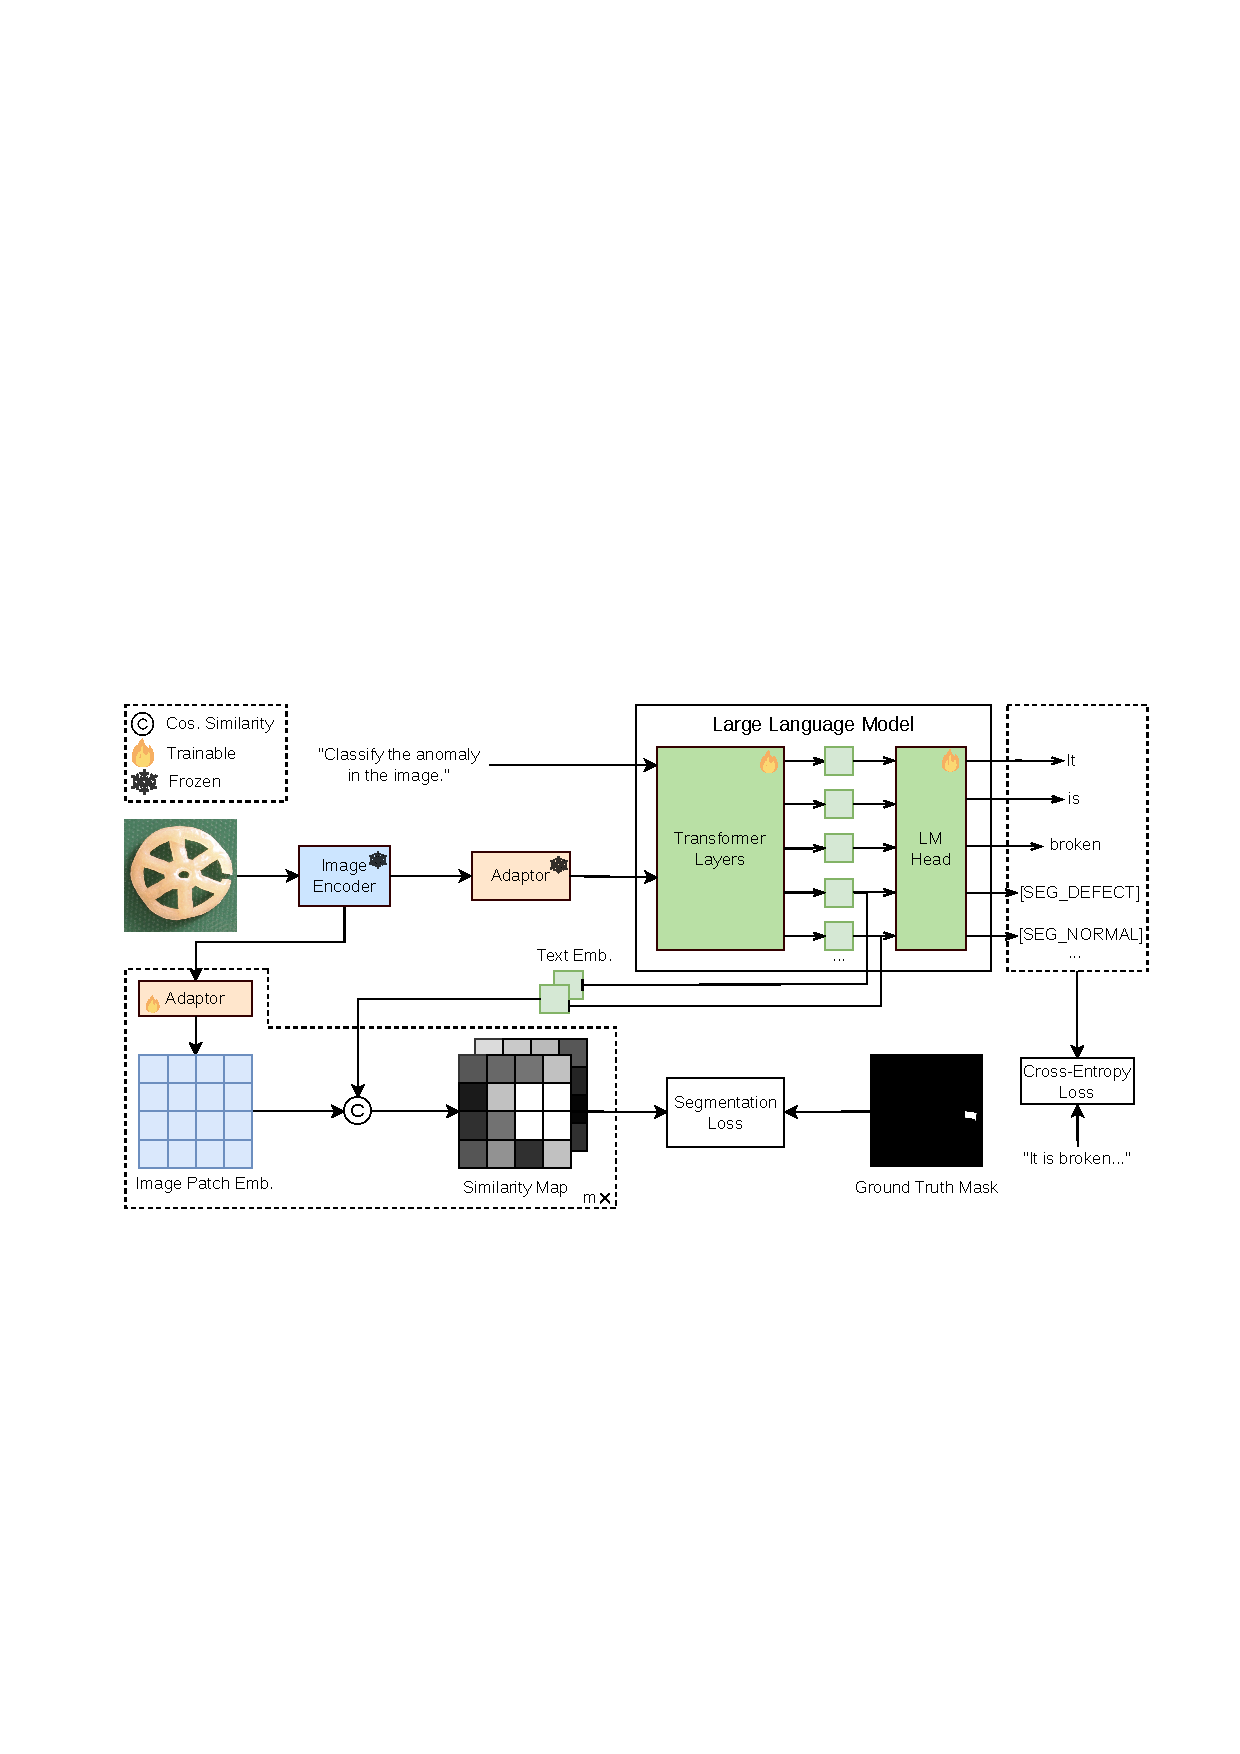
\includegraphics[width=1.0\textwidth]{imgs/GenAU_Arch_final.pdf}
  \caption[Overview of the training phase of GenAU.]{Overview of GenAU training. A frozen image encoder feeds the LLM, which generates the defect type and the \texttt{[SEG]} tokens (cross-entropy). In parallel, per-layer projections of the intermediate patch features are matched against the \texttt{[SEG]} hidden states to form the similarity map (focal + Tversky + Dice).}
   \label{fig:Model-Arch}
\end{figure*}


\subsection{Anomaly Segmentation}
\label{subsec:seg}
% The segmentation pathway computes the similarity between image and text features, inspired by prior work such as AnomalyCLIP~\cite{zhou2024anomalyclip}, MultiADS~\cite{sadikaj2025multiadsdefectawaresupervisionmultitype}, and APRIL-GAN~\cite{chen2023zero}. An image patch is classified as anomalous if its corresponding visual embedding exhibits high similarity to an anomaly-specific text embedding.
% Unlike CLIP-based models, instruction-following VLMs typically lack an explicit text encoder, making direct prompt embedding infeasible. Instead, GenAU leverages the LLM’s generative capacity to produce text embeddings conditioned jointly on the input image $\mathbf{X}_v$ and instruction $\mathbf{H}_q$. This approach allows the resulting embeddings to be contextually grounded in both the visual and linguistic input, rather than being static representations of predefined prompts. Consequently, the embeddings better capture fine-grained semantic alignment between the visual content and defect-specific textual concepts. Inspired by Lai et al.~\cite{lai2024lisareasoningsegmentationlarge}, two special tokens, \texttt{[SEG\_defect]} and \texttt{[SEG\_normal]}, are introduced into the model vocabulary. These tokens act as semantic anchors for anomalous and normal regions, respectively, and are generated immediately following the predicted defect type.
% Since the model is autoregressive, each segmentation token is conditioned on the preceding defect token, allowing the attention mechanism to encode spatial-semantic dependencies useful for segmentation. The latent representations of these tokens, extracted from the final hidden state of the LLM, serve as the anchors $\mathbf{z}^t \in \mathbb{R}^{N_z}$ for the normal and defect states.
% Each input image $\mathbf{X}_v$ is simultaneously processed by the vision encoder, which extracts patch-wise features from $m$ intermediate stages, as in APRIL-GAN~\cite{chen2023zero}. For stage $i$, the resulting feature map is $\mathbf{e}_i^p \in \mathbb{R}^{h \times w}$, where $h \times w$ denotes spatial resolution. To align the differing embedding spaces of the vision and language modalities, a set of stage-specific linear projection layers is introduced. Each layer maps its corresponding visual features into the LLM’s embedding space, producing projected features $\mathbf{z}_i^p \in \mathbb{R}^{h \times w}$.
% After projection, cosine similarity is computed between each patch embedding and both the normal and defect text embeddings to produce stage-wise similarity maps:
% $\mathbf{S}_i = \frac{\mathbf{z}_i^p}{\|\mathbf{z}_i^p\|} \cdot \frac{\mathbf{z}_i^t}{\|\mathbf{z}_i^t\|},$
% where $\mathbf{S}_i \in \mathbb{R}^{h \times w \times 2}$, and the two channels correspond to the similarity with the normal and defect descriptors, respectively.
% The similarity maps are upsampled to the input resolution and normalized across channels via softmax, yielding a per-pixel anomaly probability map. A higher activation in the anomaly channel indicates stronger confidence of defect presence.
GenAU performs anomaly localization by grounding visual features with the hidden states of generated segmentation tokens. Given an image $\mathbf{X}_v$ and an instruction $\mathbf{X}_q$, the autoregressive decoder generates a structured response containing the special tokens \texttt{[SEG\_normal]} and \texttt{[SEG\_defect]}. Let $\mathbf{h}_{\mathrm{normal}}, \mathbf{h}_{\mathrm{defect}}\in\mathbb{R}^{D}$ denote their final-layer decoder hidden states. These two vectors serve as language-grounded anchors for the normal and defective states:
Here, language-grounded denotes conditioning on the image, instruction, and preceding response through the decoder; it is not a claim that linguistic semantics alone explain the localization gain.
\begin{equation}
    \mathbf{T}
    =
    [\mathbf{h}_{\mathrm{normal}}, \mathbf{h}_{\mathrm{defect}}]
    \in \mathbb{R}^{2\times D}.
\end{equation}

The input image is processed by the frozen vision encoder to obtain multi-scale patch features from intermediate and final stages,
\(\{\mathbf{V}_i\}_{i=1}^{m}\), where
\(\mathbf{V}_i\in\mathbb{R}^{H_iW_i\times C_i}\) denotes the patch features from the \(i\)-th stage. Since the visual features and decoder hidden states lie in different representation spaces, each stage is equipped with its own \emph{linear} projection layer
\(\phi_i:\mathbb{R}^{C_i}\rightarrow\mathbb{R}^{D}\), producing
\begin{equation}
    \mathbf{Z}_i
    =
    \phi_i(\mathbf{V}_i)
    \in
    \mathbb{R}^{H_iW_i\times D}.
\end{equation}

For each stage, we compute cosine-similarity logits between every projected patch feature and the two segmentation-token anchors:
\begin{equation}
    \mathbf{S}_i
    =
    \gamma
    \cdot
    \frac{\mathbf{Z}_i}{\|\mathbf{Z}_i\|_2}
    \left(
    \frac{\mathbf{T}}{\|\mathbf{T}\|_2}
    \right)^{\top},
    \qquad
    \mathbf{S}_i\in\mathbb{R}^{H_iW_i\times 2},
\end{equation}
where \(\gamma\) is a fixed temperature scale. The two channels of \(\mathbf{S}_i\) correspond to the normal and defect scores. After reshaping \(\mathbf{S}_i\) to spatial resolution \(H_i\times W_i\), the maps are upsampled to the target mask resolution and normalized with a channel-wise softmax. The defect-channel probability gives the pixel-level anomaly map:
\begin{equation}
    \mathbf{A}_i
    =
    \mathrm{Softmax}(\mathrm{UP}(\mathbf{S}_i))_{[\mathrm{defect}]}
    \in
    [0,1]^{H\times W}.
\end{equation}
The stage-wise maps are aggregated by summation across the $m$ stages to form the final anomaly map $\mathbf{A}$, where higher values indicate a higher probability that the corresponding pixels belong to defective regions.

\paragraph{AnyRes high-resolution readout.}
The backbone encodes high-resolution inputs with an AnyRes scheme that, besides a global low-resolution view, splits the image into a grid of higher-resolution tiles. Applying the readout above to the global view alone yields a coarse low-resolution grid. To recover fine spatial detail, GenAU reassembles the patch features of the AnyRes tiles into a single high-resolution feature grid and computes the same anchor-grounded similarity maps on it. At inference, the high-resolution map $\mathbf{A}^{\mathrm{hi}}$ and the global-view map $\mathbf{A}^{\mathrm{g}}$ are fused per stage as $\mathbf{A}=(1-\beta)\,\mathbf{A}^{\mathrm{g}}+\beta\,\mathbf{A}^{\mathrm{hi}}$ with a fixed weight $\beta$. This high-resolution readout is used for all reported segmentation results.

\subsection{Image-level Anomaly Scoring}
Building on the segmentation map above, GenAU computes the image-level anomaly score without training a separate image-level classifier. Let $\mathbf{A}$ denote the final anomaly map of Section~\ref{subsec:seg} (the stage-aggregated defect response). The image-level anomaly score is its spatial maximum,
\begin{equation}
    s_{\mathrm{img}}
    =
    \max_{(u,v)}\mathbf{A}(u,v),
\end{equation}
where a larger $s_{\mathrm{img}}$ indicates a higher probability that the image contains an anomaly. This score introduces no additional trainable parameters and is obtained entirely from the language-grounded segmentation readout.

\paragraph{Fused image-level score.}
The map maximum $s_{\mathrm{img}}$ is a purely visual readout. Because the decoder additionally emits an explicit normal/defect decision, the image-level score we report is
\begin{equation}
    s_{\mathrm{fused}}
    =
    \tfrac{1}{2}\,\tilde{s}_{\mathrm{img}}
    +
    \tfrac{1}{2}\,\tilde{\ell}_{\mathrm{nd}},
\end{equation}
where $\ell_{\mathrm{nd}}$ is the decoder's normal/defect (yes/no) log-odds averaged over eight phrasings of the detection question (the question templates of the VisA and MPDD benchmarks; the image prefix is encoded once and reused), and the visual score $\tilde{s}_{\mathrm{img}}$ and $\tilde{\ell}_{\mathrm{nd}}$ are each standardized by a frozen calibration estimated once on MVTec (Appendix~\ref{app:impl}); no target-domain labels are used. Unless stated otherwise, all reported image-level results use $s_{\mathrm{fused}}$.



\subsection{Textual Reasoning and Multi-Type Anomaly Detection}
%We leverage the general-purpose visual understanding of large VLMs and adapt them for industrial anomaly detection through targeted fine-tuning on a single-label classification task. 
% The model is trained to predict the specific defect type present in an image, enabling it to capture subtle, domain-specific visual cues such as surface imperfections, texture irregularities, and localized damage that are critical for industrial inspection. 
For conditional defect-type recognition, GenAU receives a known-anomalous target image $\mathbf{X}_v$ and an instruction listing its object's coarse candidate labels $C_{\mathrm{target}}(o)$. It generates a response $\mathbf{X}_a$; a deterministic parser $\pi(\cdot)$ selects one label $\hat{y}'\in C_{\mathrm{target}}(o)$, or an unmatched sentinel counted as an error (Appendix~\ref{app:eval}). Compound labels represent combinations as one class, rather than independent per-type predictions.
% Thus, instead of learning a fixed classifier over $C_{\mathrm{train}}$, GenAU formulates multi-type anomaly detection as constrained conditional generation over $C_{\mathrm{target}}$, preserving language reasoning while producing domain-specific, machine-readable predictions.

\subsection{Training Objective}

GenAU is optimized with a joint objective that supervises textual reasoning and pixel-level anomaly segmentation. For each training sample, the model receives an image $\mathbf{X}_v$ and an instruction $\mathbf{X}_q$, and is trained to generate a structured response $\mathbf{X}_a=(a_1,\ldots,a_T)$ containing the predicted defect type and the grounding tokens \texttt{[SEG\_normal]} and \texttt{[SEG\_defect]}. The overall objective is
\begin{equation}
    \mathcal{L}
    =
    \mathcal{L}_{\mathrm{txt}}
    +
    \lambda_{\mathrm{seg}}\mathcal{L}_{\mathrm{seg}},
    \label{eq:overall-loss}
\end{equation}
where $\lambda_{\mathrm{seg}}$ balances the language-modeling and pixel-level supervision terms. The image-level anomaly score is computed at inference from the segmentation map and the decoder's yes/no log-odds (Sec.~\ref{subsec:seg}) and thus requires no dedicated training term.

\paragraph{Text generation loss.}
The textual reasoning objective is the standard autoregressive cross-entropy loss over the target response tokens:
\begin{equation}
    \mathcal{L}_{\mathrm{txt}}
    =
    -
    \sum_{t=1}^{T}
    \log
    p_{\theta}
    \left(
        a_t
        \mid
        a_{<t}, \mathbf{X}_v, \mathbf{X}_q
    \right).
    \label{eq:text-loss}
\end{equation}
This term trains the model to generate domain-specific inspection responses, including defect-type descriptions and the required segmentation tokens. Prompt tokens and inserted visual tokens are excluded from the language modeling loss.

\paragraph{Pixel-level segmentation loss.}
For anomaly segmentation, GenAU predicts stage-wise similarity maps $\{\mathbf{S}_i\}_{i=1}^{m}$, where each $\mathbf{S}_i$ contains normal and defect logits for visual patches at stage $i$. Let $\mathbf{A}_i$ and $\mathbf{A}_i^{\mathrm{n}}$ denote the defect- and normal-channel probability maps after upsampling and channel-wise softmax. Given a binary ground-truth mask $\mathbf{M}_x\in\{0,1\}^{H\times W}$, the segmentation loss is summed over all visual stages:
\begin{align}
    \mathcal{L}_{\mathrm{seg}}
    =
    \sum_{i=1}^{m}
    \Big(
        &
        \mathcal{L}_{\mathrm{focal}}
        \big(
            \mathrm{UP}(\mathbf{S}_i),
            \mathbf{M}_x
        \big)
        +
        \mathcal{L}_{\mathrm{Tversky}}
        \big(
            \mathbf{A}_i,
            \mathbf{M}_x
        \big)
        \notag \\
        &
        +
        \mathcal{L}_{\mathrm{dice}}
        \big(
            \mathbf{A}_i^{\mathrm{n}},
            \mathbf{1}-\mathbf{M}_x
        \big)
    \Big).
    \label{eq:seg-loss}
\end{align}
The focal term mitigates the severe foreground/background imbalance; the Tversky term on the defect channel up-weights false negatives over false positives, improving region recall and AUPRO; and the Dice term on the normal channel suppresses false positives. For anomalous images $\mathbf{M}_x$ is the annotated mask; for normal images it is all-zero, giving negative supervision.

\paragraph{Trainable parameters.}
We use parameter-efficient fine-tuning: the vision encoder stays frozen, while the cross-modal projector, LoRA~\cite{hu2021loralowrankadaptationlarge} on the decoder, the token-embedding table and LM head (for the two segmentation tokens), the $m$ stage-wise projectors $\{\phi_i\}$, and the decoder layer-norms are trained jointly under Eq.~\ref{eq:overall-loss}.
% To jointly optimize the model for textual reasoning and visual localization, we employ a composite objective combining text generation and segmentation supervision. The overall loss is defined as:
% \begin{align}
% \mathcal{L} =  \mathcal{L}_\text{txt} + \lambda_1 \mathcal{L}_\text{seg} + \lambda_2 \mathcal{L}_\text{img}, \label{eq:overall-loss}
% \end{align}
% where $L_{txt}$ is the autoregressive cross-entropy loss for text generation:
% \begin{align}
%  \mathcal{L}_\text{txt} =  \mathcal{L}_\text{CE}(\hat{y}_\text{txt}, y_\text{txt}), \label{eq:ce}
% \end{align}
% with $\hat{y}_{txt}$ representing the predicted token distribution and $y_{txt}$ the ground-truth token. The cross-entropy loss is the standard objective for sequence generation tasks and ensures accurate prediction of the defect type and segmentation tokens.

% The segmentation loss $L_{seg}$ encourages precise localization and is computed as a combination of focal and dice losses across all $m$ feature stages:
% \begin{align}
% \mathcal{L}_\text{seg}
% = \sum_{i=1}^{m} \Big(
% 	&\mathcal{L}_\text{focal}(UP(\mathbf{S}_i), \mathbf{M}_x) \notag \\
% 	&+ \mathcal{L}_\text{dice}(UP(\mathbf{S}_i[1]), \mathbf{M}_x)
% \Big).
% \label{eq:Loss}
% \end{align}
% where $\mathbf{M}_x$ is the binary ground truth mask, $UP(\cdot)$ denotes upsampling function, and $\mathbf{S}_i[1]$ corresponds to the anomaly channel. Focal loss is employed to mitigate the severe class imbalance between normal and defective pixels, while the dice loss promotes better overlap between the predicted segmentation and the ground-truth mask, improving boundary precision and region consistency.


% \subsection{Training Data Formulation}
% Training data are derived from established anomaly detection and segmentation benchmarks~\cite{Bergmann_2019_CVPR, VisA, wang2024realiadrealworldmultiviewdataset}.
% We retain the original images and segmentation masks from these datasets and augment them by introducing instruction-response pairs specifically designed for instruction-tuned training.
% Each training sample thus consists of the original image, its segmentation mask, a newly added textual instruction, and a corresponding response.
% The instruction prompts the model to identify the defect present in the image and enumerates the possible defect types for that object category, while the response specifies the correct defect type followed by the segmentation tokens.
% This augmentation step is the only modification to the original datasets and enables the model to learn the association between visual anomalies and structured textual outputs. 
% Each prompt follows a structured format comprising: (1) a request to identify the defect, (2) a text description of normal appearance, and (3) definitions of potential defect types. This design embeds domain knowledge similar to how human inspectors reason about faults. An example description for a \textit{contamination} defect on a tile object would be similar to:

% \textit{``Contamination: The presence of any unwanted foreign material, substance, or object on the surface or inside the item. This can include debris, spots, smudges, particles, threads, metal, or other materials. For this surface, contamination manifests as translucent or yellowish oil spots, glue strips, or small plastic fragments distinct from the tile’s natural pattern.''}

% The expected model response includes a Chain-of-Thought (CoT) reasoning that describes its decision process and concludes with the final classification:

% \textit{``I am inspecting the tile for the following defects: Crack, Contamination, Scratch, Color. The surface is solid and unscratch\-ed; color is normal; a foreign plastic piece is visible. This matches the definition of Contamination.
% Final Answer: Contamination [SEG\_defect] [SEG\_normal].''}

% Industrial AD datasets often define highly specific defect categories, which can lead to overfitting and inconsistent label usage~\cite{mokhtar2025detectclassifyactcategorizing}.
% To improve generalization, we create a unified defect taxonomy, similar to  MultiADS~\cite{sadikaj2025multiadsdefectawaresupervisionmultitype}. Product-specific labels are mapped to broader semantic groups, e.g., \textit{liquid} and \textit{metal contamination} are merged into \textit{contamination}, and \textit{broken large} and \textit{broken small} are unified as \textit{broken}. The complete taxonomy mapping is provided in the Appendix.
% This reclassification simplifies learning, promotes abstraction over product-specific anomalies, and mitigates data imbalance. Importantly, it does not affect comparisons with prior methods, as their AD metrics are binary and independent of class granularity.

% \subsection{Trainable Parameters}
% To efficiently adapt large instruction-following VLMs while preserving their pretrained knowledge, GenAU employs a parameter-efficient LoRA~\cite{hu2021loralowrankadaptationlarge} fine-tuning strategy on the LLM backbone.
% The embedding layer and language modeling head are fully fine-tuned to integrate the newly introduced segmentation tokens into the model’s vocabulary.
% In contrast, the vision encoder and the original cross-modal projection layer connecting it to the LLM are kept frozen, to preserve its pre-trained visual-semantic alignment learned on large-scale image-text data.
% Only the lightweight LoRA parameters within the LLM and the additional stage-wise projection layers for visual-text alignment are trainable.
% This setup minimizes computational overhead and memory usage while maintaining strong cross-modal correspondence between the visual and textual representations.

% \subsection{Inference}
% During inference, the model operates autoregressively, generating the textual output token by token to predict one or more defect types. When the segmentation tokens are produced, their latent embeddings are extracted and used as text queries to compute similarity with the multi-scale visual features, following the same procedure as during training.
% The resulting similarity maps from all encoder stages are combined through element-wise summation to yield the final anomaly map.

% In parallel, the model produces an image-level anomaly score $a_x$, defined as the maximum activation in the anomaly channel. This score provides a quantitative measure of defect presence, complementing the text-based defect classification and enabling unified evaluation of both binary detection and segmentation performance.

\subsection{Inference}
For binary detection and segmentation, the instruction names the object category and asks \texttt{``Is there any anomaly on the \{object\}? If yes, segment it.''} Image-level scoring averages decoder yes/no log-odds over eight phrasings, reusing the image encoding. Conditional type recognition instead states that the image contains a defect and lists the object's candidate coarse labels: \texttt{``Identify the defect type. Choose exactly one option from this list: \{defect list\}.''}

For detection and segmentation, the generated answer is followed by the two segmentation tokens. If they are omitted, we append them and read their hidden states with one additional forward pass, so every image receives a map independent of the textual normal/defect decision. Binary detection uses $s_{\mathrm{fused}}$; segmentation uses the AnyRes-fused map, with all-zero supervision on normal training images. Type recognition uses its separate forced-choice prompt and parser, and reasoning uses the conversational questions of VisA-D\&R. The same checkpoint can serve all four tasks, but these are separate task-conditioned evaluations, not necessarily one joint response per image.


\section{Experiments}

\subsection{Datasets}
We use four public industrial anomaly benchmarks (MVTec-AD~\cite{Bergmann_2019_CVPR}, VisA~\cite{VisA}, MPDD~\cite{mpdd}, and Real-IAD~\cite{wang2024realiadrealworldmultiviewdataset}), plus VisA-D\&R~\cite{xu2025towards} for defect reasoning, covering the three tasks of Sec.~\ref{sec:prelims} and defect reasoning/analysis. Additional details are in Appendix.

\subsection{Experimental Settings}
We build GenAU on LLaVA-OneVision~\cite{li2025llavaonevision}, which pairs a Qwen2 language backbone with a frozen SigLIP-so400m-patch14-384 vision encoder, and report results at the 0.5B and 7B scales. Following prior zero-shot protocols~\cite{sadikaj2025multiadsdefectawaresupervisionmultitype, chen2023zero, zhou2024anomalyclip}, GenAU is fine-tuned on the test split of MVTec-AD (its only split carrying anomaly masks and defect-type labels, the train split being normal-only) and evaluated, without retraining, on VisA, MPDD, and Real-IAD; MVTec-AD is thus purely the source domain and is disjoint from every evaluation target.
High-resolution inputs use AnyRes (\texttt{anyres\_max\_9}, up to a $6\times6$ grid of $384$-px tiles); the segmentation readout reassembles the tiles into a high-resolution feature grid, fused with the global view ($\beta=0.25$, temperature $20$) using patch features from vision-encoder layers $6,12,18,27$. We adapt only LoRA~\cite{hu2021loralowrankadaptationlarge} ($r=16$, $\alpha=32$) on the LLM, the token embeddings and LM head (to add the two segmentation tokens), the cross-modal projector, and the per-stage projectors and decoder layer-norms; only the encoder stays frozen. For half of the $1{,}725$ training images the segmentation exchange is part of a multi-turn reasoning conversation~\cite{xu2025towards}; each image appears once, so training keeps $53$ steps (Appendix~\ref{app:data}). The segmentation loss combines focal, Tversky ($\alpha=0.3$, $\beta=0.7$), and Dice, with $\lambda=1$ (Eq.~\ref{eq:overall-loss}) and no separate image-level loss; the image score is the fused score $s_{\mathrm{fused}}$ of Sec.~\ref{subsec:seg}. We train one epoch at effective batch size $32$ ($lr=10^{-4}$ cosine, warmup $0.03$, no weight decay; $8$ GPUs, ZeRO-3). All tasks use one checkpoint per scale, with no weight changes between tasks. Further details, including the multi-type prompt and parser, are in Appendix.

\subsection{Evaluation Metrics}
We report image-level AUROC and AP for detection; pixel-level AUROC and AUPRO for segmentation; weighted Precision/Recall/F1 for multi-type detection (to handle class imbalance); and, for reasoning, the VisA-D\&R GPT-Score~\cite{xu2025towards}, where GPT-4o rates each response $1$--$10$ for low-level (perception) and complex (causal-reasoning) questions separately (full definitions in Appendix).

\subsection{Baselines}
All baselines, like GenAU, access only the query image at test time: no reference, support, or exemplar images. As \emph{CLIP-based} zero-shot detectors and segmenters we compare against CLIP, CLIP-AC~\cite{radford2021}, WinCLIP~\cite{jeong2023winclip}, APRIL-GAN~\cite{chen2023zero}, CoOp~\cite{CoOp}, CoCoOp~\cite{zhou2022conditionalpromptlearningvisionlanguage}, AnomalyCLIP~\cite{zhou2024anomalyclip}, AdaCLIP~\cite{Cao_2024}, FiLo~\cite{gu2024filozeroshotanomalydetection}, and MultiADS together with its variant MultiADS-F~\cite{sadikaj2025multiadsdefectawaresupervisionmultitype}, the only CLIP-based baseline that additionally performs multi-type detection. For the multi-type and reasoning tasks we further compare against \emph{vision--language} baselines: the anomaly-reasoning specialist Anomaly-OV~\cite{xu2025towards} and our LLaVA-OneVision~\cite{li2025llavaonevision} backbone, both at the $0.5$B and $7$B scales. Methods without public implementations (e.g., SimCLIP~\cite{simclip}) are excluded for reproducible comparison.

\subsection{Results}
Next, we present and discuss results for binary anomaly detection and segmentation under distribution shift, multi-type zero-shot anomaly detection, and defect reasoning, the four tasks GenAU addresses within a single model.
\subsubsection{Binary Detection and Segmentation under Distribution
Shift}
Table~\ref{tab:binary} reports the performance of GenAU on VisA, MPDD, and Real-IAD, compared with state-of-the-art CLIP-based methods. Pixel-level metrics (AUROC, AUPRO) and image-level metrics (AUROC, AP) are reported.

On VisA, the 7B model achieves the best image-level AUROC ($90.1\%$) among the methods in Table~\ref{tab:binary}; the VLM reasoning specialist Anomaly-OV-7B reports a VisA image-AUROC of $88.9\%$ but is trained under an instruction-tuning rather than our cross-dataset protocol and produces no segmentation, so we note it here only for context. On MPDD, GenAU-7B attains the highest pixel-level AUROC and AUPRO ($96.7\%$, $89.8\%$) and image-level AP ($85.1\%$), while its image-level AUROC ($78.7\%$) stays below MultiADS-F ($79.7\%$), reflecting the logical and large-area anomalies of this dataset. On Real-IAD, it reaches an image-level AUROC of $85.1\%$ and the highest pixel-level AUPRO ($88.2\%$). Its pixel-level scores on VisA, however, remain below the strongest CLIP-based segmenters. The 0.5B variant remains competitive, with the second-best image-level AUROC on VisA and Real-IAD.
Overall, GenAU demonstrates that a single instruction-following VLM can achieve strong binary detection and segmentation performance under distribution shift.
\begin{table}
\setlength{\tabcolsep}{2pt}
\centering
	\caption[Results of GenAU for binary anomaly detection and segmentation under distribution shift]{Zero-shot binary detection and segmentation under distribution shift (\%). \textbf{Bold}/\underline{underline}: best/second best. Baseline numbers are quoted from MultiADS~\cite{sadikaj2025multiadsdefectawaresupervisionmultitype} and FiLo~\cite{gu2024filozeroshotanomalydetection} and are \emph{not} recomputed in our harness.}
	\label{tab:binary}
\begin{tabular}{c|ccccc}
\toprule
\multirow{2}{*}{\textbf{Dataset}} & \multirow{2}{*}{\textbf{Method}}  
& \multicolumn{2}{c}{\textbf{Pixel-Level}} & \multicolumn{2}{c}{\textbf{Image-Level}} \\
\cmidrule{3-6}
& & \textbf{AUROC} & \textbf{AUPRO} & \textbf{AUROC} & \textbf{AP} \\
\midrule
\multirow{13}{*}{VisA}
& CLIP        & 46.6 & 14.8 & 66.4 & 71.5 \\
& CLIP-AC     & 47.8 & 17.3 & 65.0 & 70.1 \\
& CoOp        & 24.2 & 3.8 & 62.8 & 68.1 \\
& CoCoOp      & 93.6 & - & 78.1 & - \\
& WinCLIP     & 79.6 & 56.8 & 78.1 & 81.2 \\
& APRIL-GAN   & 94.2 & 86.8 & 78.0 & 81.4 \\
& AnomalyCLIP  & \underline{95.5} & 87.0 & 82.1 & 85.4 \\
& AdaCLIP     & 95.0 & - & 75.4 & 79.3 \\
& FiLo     & \textbf{95.9} & - & 83.9 & - \\
& MultiADS   & 95.0 & \textbf{89.7} & 83.6 & 86.9\\
& MultiADS-F & 94.5 & 87.4 & 82.5 & 86.5 \\
\cmidrule(lr){2-6}
% 2026-10-17: GenAU rows = halfmix checkpoints (hires-tversky{,-05b}-halfmix-proj), runs halfmix-{7b,05b}-<ds>-fair,
% fused with their own MVTec calibration (evaluation/fusion_calib_halfmix{,05b}_ens8.json).
&  GenAU-0.5b &      95.0 & \underline{88.2} & \underline{89.2} & \underline{90.9} \\
&  GenAU-7b &      94.4 & 87.4 & \textbf{90.1} & \textbf{91.8} \\
\midrule
\multirow{12}{*}{MPDD}
& CLIP        & 62.1 & 33.0 & 54.3 & 65.4 \\
& CLIP-AC     & 58.7 & 29.1 & 56.2 & 66.0 \\
& CoOp        & 15.4 & 2.3  & 55.1 & 64.2 \\
& CoCoOp      & 95.2 & - & 61.0 & - \\
& WinCLIP      & 76.4 & 48.9 & 63.6 & 69.9 \\
& APRIL-GAN    & 94.1 & 83.2 & 73.0 & 80.2 \\
& AnomalyCLIP  & 96.5 & 88.7 & 77.0 & 82.0 \\
& AdaCLIP      & 96.3 & - & 66.3 & 75.0 \\
& MultiADS   & 95.8 & \underline{89.7} &  78.3 & 78.4 \\
& MultiADS-F & 96.3 & 89.5 & \textbf{79.7} & 80.5 \\
\cmidrule(lr){2-6}
& GenAU-0.5b &   \underline{96.6} & 88.1 & 76.2 & \underline{82.6} \\
& GenAU-7b &       \textbf{96.7} & \textbf{89.8} & \underline{78.7} & \textbf{85.1} \\
\midrule
\multirow{8}{*}{Real-IAD} 
& WinCLIP      & 87.1 & 59.9 & 75.0 & 72.3 \\
& APRIL-GAN    & 96.0 & 86.8 & 75.7 & 73.5 \\
& AnomalyCLIP  & 96.2 & 85.7 & 78.4 & 76.7 \\
& AdaCLIP      & 95.3 & - & 70.1 & 68.5 \\
& MultiADS   & \textbf{96.6} & 87.1 & 78.7 & 79.1\\
& MultiADS-F   &  \underline{96.3} & \underline{87.2} & 78.2 & 78.5 \\
\cmidrule(lr){2-6}
& GenAU-0.5b &        89.5 & 75.1 & \underline{84.3} & \underline{84.9}\\
& GenAU-7b &        \underline{96.3} & \textbf{88.2} & \textbf{85.1} & \textbf{85.4}\\
\bottomrule
\end{tabular}
\end{table}
Qualitative results of GenAU and the best overall performer, MultiADS, are shown in Figure~\ref{fig:visa-visual-good} (and, for a failure case, Figure~\ref{fig:visa-visual-bad}). GenAU accurately segments visually salient defects such as \textit{hole}, \textit{broken}, and \textit{crack}, and produces cleaner, lower-noise segmentation maps than MultiADS. However, global-context or logic-dependent defects such as \textit{missing} components remain challenging. For these cases, similarity maps are low-confidence, often resulting in incomplete localization or misclassification of normal regions for both models (Figure~\ref{fig:visa-visual-bad}).

\begin{figure}[h]
  \centering
  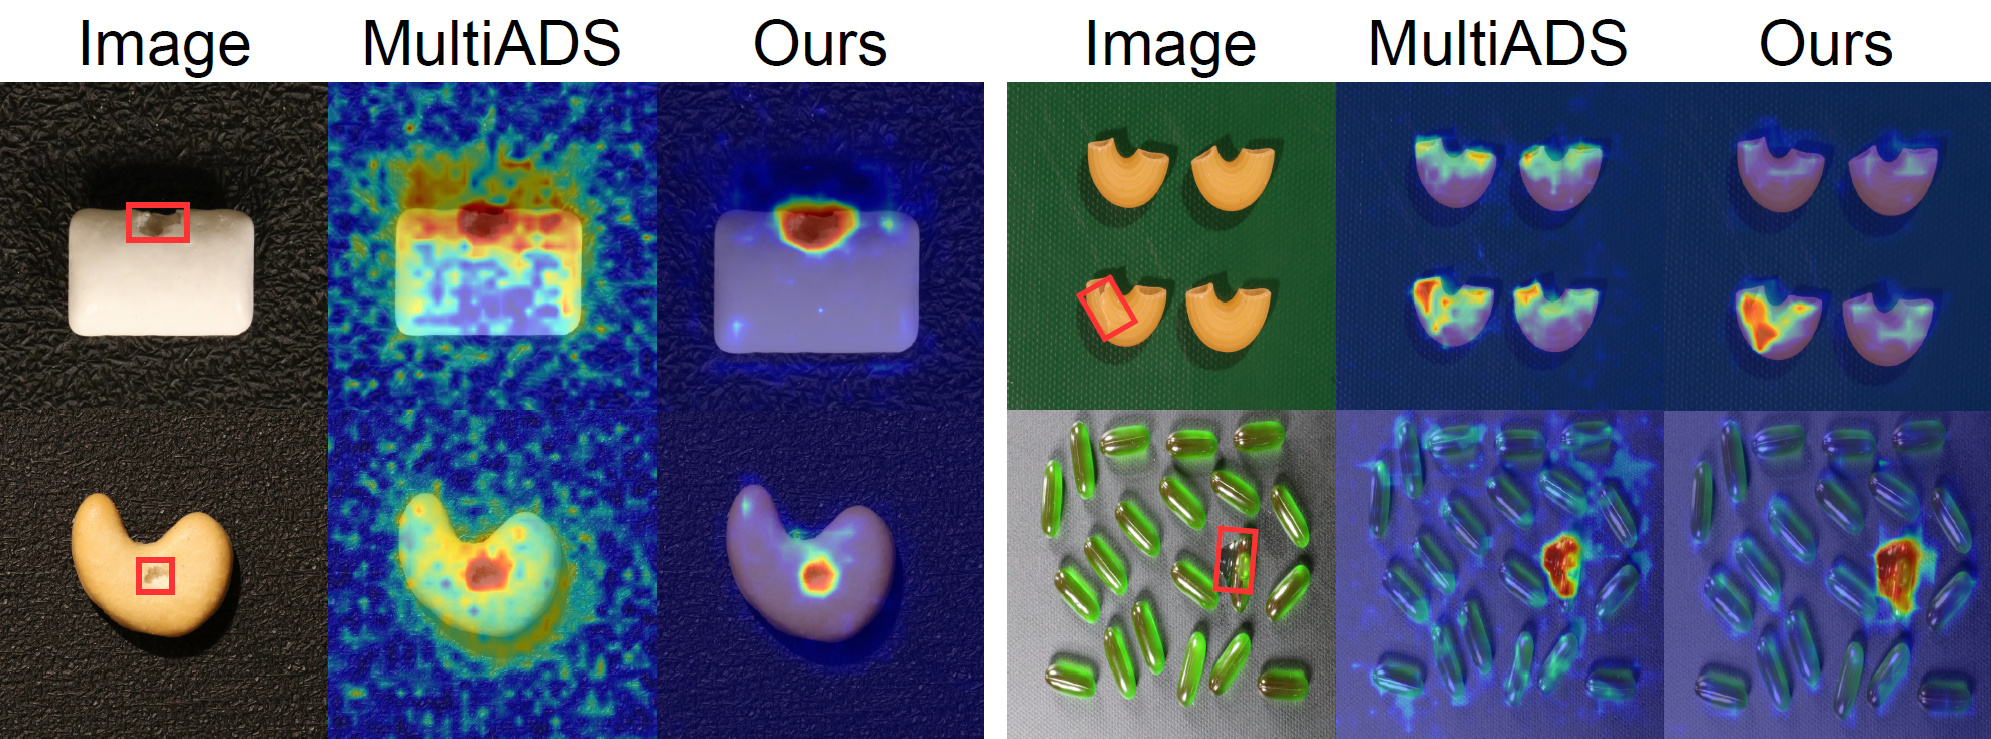
\includegraphics[width=1.0\columnwidth]{imgs/Visa-visual.jpg}
  \caption{Visualization of anomaly segmentation under distribution shift from VisA. Results are compared with MultiADS.}
   \label{fig:visa-visual-good}
\end{figure}

\textbf{Ablation Studies}.\label{sec:ablations}
Replacing decoder-conditioned anchors with randomly initialized, trainable constant queries lowers VisA pixel-AUPRO from $88.7$ to $87.4$ (Table~\ref{tab:ablations_main}). Under matched inference, decoder anchors improve pixel-AUPRO by $1.28$ points on VisA and $0.19$ on MPDD, but trail by $1.78$ on Real-IAD. Across three training seeds, the mean differences are $+4.40$, $-0.47$, and $-0.68$ points, respectively: the localization benefit is dataset-dependent, not universal. Both arms produce maps for every image, using the appended-token fallback when needed.
Table~\ref{tab:ablations_main} varies one factor at a time on VisA. Removing the LM fusion (\emph{map-max only}) lowers image-AUROC by $5.6$ points ($90.1\!\rightarrow\!84.5$); fusing the log-odds of only the single question an image is asked recovers $2.2$ of them ($86.7$), so averaging over phrasings supplies most of the gain. The VLM prior is useful by itself: untrained LLaVA-OneVision, asked the same eight questions, reaches $87.0$ image-AUROC from its yes/no log-odds alone, above every CLIP baseline in Table~\ref{tab:binary} (on Real-IAD, $84.4$ versus $78.7$); fine-tuning raises this term to $89.2$. Training on segmentation alone, at the same $53$ steps, adds $1.8$ pixel-AUPRO but no detection, and segmentation-only checkpoints answer complex VisA-D\&R questions poorly (SBERT similarity $0.576$ versus $0.664$; Appendix~\ref{app:eval}). Giving every training image a reasoning conversation (\emph{full reasoning mix}) instead doubles the optimization steps and costs $3.5$ image-AUROC and $2.9$ pixel-AUPRO, so our default embeds reasoning in half of the samples at an unchanged budget. Freezing the LLM decoder -- keeping the adapter attached but untrained -- leaves detection and localization nearly unchanged ($90.0$ image-AUROC, $88.0$ AUPRO), but the frozen decoder rarely emits the segmentation tokens on its own (they are appended for $1{,}984$ of $2{,}162$ VisA images): adapting the decoder lets the model request segmentation itself, rather than improving the readout or the decision. The ablation studies of hyper-parameters are in Appendix.

\begin{table}
\small
\centering
\setlength{\tabcolsep}{3pt}
\caption{GenAU-7B ablations on VisA (\%). The shaded row is our default; each indented row changes one factor of the nearest less-indented row above it. $^\ast$Also halves the text-loss weight. Image columns use the fused score of Table~\ref{tab:binary}.}
\label{tab:ablations_main}
\begin{tabular}{@{}l|cc|cc@{}}
\toprule
 & \multicolumn{2}{c|}{\textbf{Pixel}} & \multicolumn{2}{c}{\textbf{Image}} \\
\cmidrule(lr){2-3}\cmidrule(lr){4-5}
 & AUROC & AUPRO & AUROC & AP \\
\midrule
% 2026-10-07: every row re-evaluated with the appended-token inference step (SEG_FORCE_ANCHORS=1,
% evaluation_summary_*-fair). The comments below describe the earlier, pre-fix values.
% 2026-10-10: image columns = fused score with the 8-phrasing LM term (evaluation/fusion_calib_tversky_ens8.json,
% w=1), from evaluation/lm_decision/<tag>-visa_s*.npz + per_sample_<run>.jsonl; same frozen calibration on every row.
% 2026-10-17 (halfmix default). Default + w/o fusion + single-question: halfmix-7b-visa-fair with its own calibration
% (fusion_calib_halfmix_ens8.json; single question: assigned-question log-odds, MVTec-standardized, w=0.5).
% segmentation only = noreason-proj (trainable projector); frozen projector = the earlier default hires-tversky-1layer-1ep-bs32.
% These rows use fusion_calib_tversky_ens8.json. frozen LLM = noreason-proj-lm05-nolora-s42 (projector trained, LM-loss weight 0.5).
% LQA image columns: 8-phrasing dump job 5190332 (single-question score was 86.7 / 89.1).
\rowcolor{gray!20}
GenAU-7B (default) & 94.4 & 87.4 & 90.1 & 91.8 \\
\midrule
\quad w/o LM fusion & 94.4 & 87.4 & 84.5 & 87.6 \\
\quad single-question LM term & 94.4 & 87.4 & 86.7 & 89.2 \\
\quad segmentation only & 95.6 & 89.2 & 89.9 & 91.5 \\
\qquad frozen LLM$^\ast$ & 95.2 & 88.0 & 90.0 & 91.7 \\
\qquad frozen projector & 95.1 & 88.7 & 90.5 & 91.9 \\
\qquad\quad learned-query anchors & 94.3 & 87.4 & 89.0 & 90.9 \\
\qquad\quad full reasoning mix & 95.1 & 85.8 & 87.0 & 89.6 \\
\midrule
% Base LLaVA-OV-7B, no anomaly training: mean yes/no log-odds over the 8 phrasings only (evaluation/lm_decision/base-visa_s*.npz).
untrained LLaVA-OV, LM only & -- & -- & 87.0 & 89.4 \\
\bottomrule
\end{tabular}
\end{table}


\subsubsection{Zero-Shot Multi-Type Detection}
We evaluate candidate-list-conditioned defect-type classification on known-anomalous images of VisA and MPDD (Table~\ref{tab:multytype_zero_shot_detection_performance}). The prompt supplies the target object's possible coarse defect labels and asks for one label; compound defects may form a \emph{combined} class, rather than being decoded as multiple independent labels. This is conditional type recognition, not joint normal/anomalous and multi-label prediction. The mapped evaluation subsets contain $916$ VisA and $282$ MPDD images; unmapped labels are excluded (Appendix~\ref{app:eval}).
GenAU-7B, the checkpoint of Table~\ref{tab:binary}, obtains weighted F1 of $33.4\%$ and $89.5\%$, respectively, the highest values in this table. Three of the six MPDD objects have a single candidate label, so an oracle predicting each object's most frequent label already reaches $76.0\%$ there ($31.4\%$ on VisA). Anomaly-OV-0.5B/7B are our MVTec-trained reproductions with a two-turn detect-then-classify prompt. MultiADS, designed for multi-type segmentation, is converted to detection by thresholding its per-type channels at $0.5$; its comparison is therefore operating-point-dependent, not evidence of superiority under an optimized threshold. VisA's finer, object-dependent taxonomy remains difficult despite its higher precision.

\begin{table}
\small
\centering
\caption[Conditional defect-type recognition.]{Conditional defect-type recognition on mapped anomalous images (\%). GenAU uses the checkpoints of Table~\ref{tab:binary}; the prompt and scorer exclude normal as an option. \textbf{Bold}: highest reported value per column. Anomaly-OV uses our MVTec-trained two-turn reproductions; MultiADS uses a fixed $0.5$ channel threshold.}
\label{tab:multytype_zero_shot_detection_performance}
\begin{tabular}{@{}llccc@{}}
\toprule
\textbf{Dataset}          & \textbf{Model} & \textbf{Precision} & \textbf{Recall} & \textbf{F1} \\ \midrule
\multirow{5}{*}{VisA}     & MultiADS         & 17.4          & \textbf{57.7} & 18.6          \\
                          & Anomaly-OV-0.5b  & 18.4          & 11.1          & 9.3           \\
                          & Anomaly-OV-7b  & 42.1          & 30.9          & 21.1           \\
                          \cline{2-5}
% 2026-10-17: halfmix checkpoints, runs halfmix-{05b,7b}-{visa,mpdd}-mtype-nn, score_multitype.py --no-normal.
% Segmentation-only checkpoints gave 0.5b 20.3/21.5/16.4, 18.7/30.5/23.2 and 7b 51.3/42.6/37.4, 92.7/87.9/89.2.
                          & GenAU-0.5b         & 31.1 & 20.9          & 13.8 \\
                          & GenAU-7b         & \textbf{52.4} & 38.3          & \textbf{33.4} \\ \midrule
\multirow{5}{*}{MPDD}     & MultiADS         & 34.0          & 51.3          & 32.7          \\
                          & Anomaly-OV-0.5b  & 60.1          & 30.5           & 29.9          \\
                          & Anomaly-OV-7b  & 87.1          & 65.8           & 65.1          \\
                          \cline{2-5}
                          & GenAU-0.5b         & 42.3 & 54.6          & 46.8 \\
                          & GenAU-7b         & \textbf{91.5} & \textbf{89.4} & \textbf{89.5} \\
% \multirow{1}{*}{Real-IAD}  
%                           & GenAU-7b   & 39.1               & 36.6            & 31.3      
\bottomrule
\end{tabular}
\end{table}



\subsubsection{Defect Reasoning and Analysis}
Beyond detecting and localizing defects, GenAU answers open-ended questions about them. We evaluate on VisA-D\&R~\cite{xu2025towards} (low-level perception and complex causal-reasoning questions) against the reasoning specialist Anomaly-OV~\cite{xu2025towards}; here GenAU augments its segmentation training with a reasoning instruction mix, so one model both localizes and explains, whereas Anomaly-OV produces no segmentation.

Table~\ref{tab:reasoning} gives the reported GPT-Scores. The LLaVA-OneVision and Anomaly-OV numbers are taken from~\cite{xu2025towards}, not rejudged alongside GenAU, so these comparisons are indicative rather than controlled. In particular, the $6.43$ versus $6.34$ complex-reasoning scores do not establish a reliable advantage without a shared judge and uncertainty estimates. Textual plausibility or reference agreement also does not establish the correctness of a causal diagnosis.

\begin{table}
\small
\centering
\setlength{\tabcolsep}{6pt}
\caption{Defect reasoning on VisA-D\&R~\cite{xu2025towards}, scored by GPT-4o on a $1$--$10$ scale. VisA-D\&R poses two question categories per image: \emph{Low-level} perception questions, which ask the model to describe the anomaly, and \emph{Complex} causal-reasoning questions about its significance, likely cause, and prevention; we report the GPT-Score separately for each. $^\dagger$LLaVA-OV and Anomaly-OV scores as reported in the Anomaly-OV paper~\cite{xu2025towards}. For this task GenAU augments its segmentation training with a reasoning instruction mix, and is evaluated as a single model that both localizes and explains anomalies.}
\label{tab:reasoning}
% TODO(GPT-Score): the GenAU rows, this caption and the paragraph above still describe the REASONING-MIX checkpoints.
% Replace with the user's GPT-4o scores of evaluation/gpt_score_input/visa-dr_halfmix-{7b,05b}.json (the Table 1 halfmix checkpoints).
\begin{tabular}{@{}lcc@{}}
\toprule
\multirow{2}{*}{\textbf{Model}} & \multicolumn{2}{c}{\textbf{GPT-Score}} \\
\cmidrule(lr){2-3}
 & \textbf{Low-level} & \textbf{Complex} \\
\midrule
LLaVA-OV-0.5B$^\dagger$   & 2.54 & 4.34 \\
LLaVA-OV-7B$^\dagger$     & 3.57 & 5.44 \\
Anomaly-OV-0.5B$^\dagger$ & 3.87 & 5.67 \\
Anomaly-OV-7B$^\dagger$   & 4.26 & 6.34 \\
\cmidrule(lr){1-3}
GenAU-0.5B & 5.01          & 6.13          \\
GenAU-7B   & 5.22 & 6.43 \\
\bottomrule
\end{tabular}
\end{table}


\section{Discussion}
This section provides the performance analyses of GenAU, highlighting challenges and insights that are often unexplored in prior studies.

\subsection{Local vs. Global Context Segmentation}
\begin{figure}[t]
  \centering
  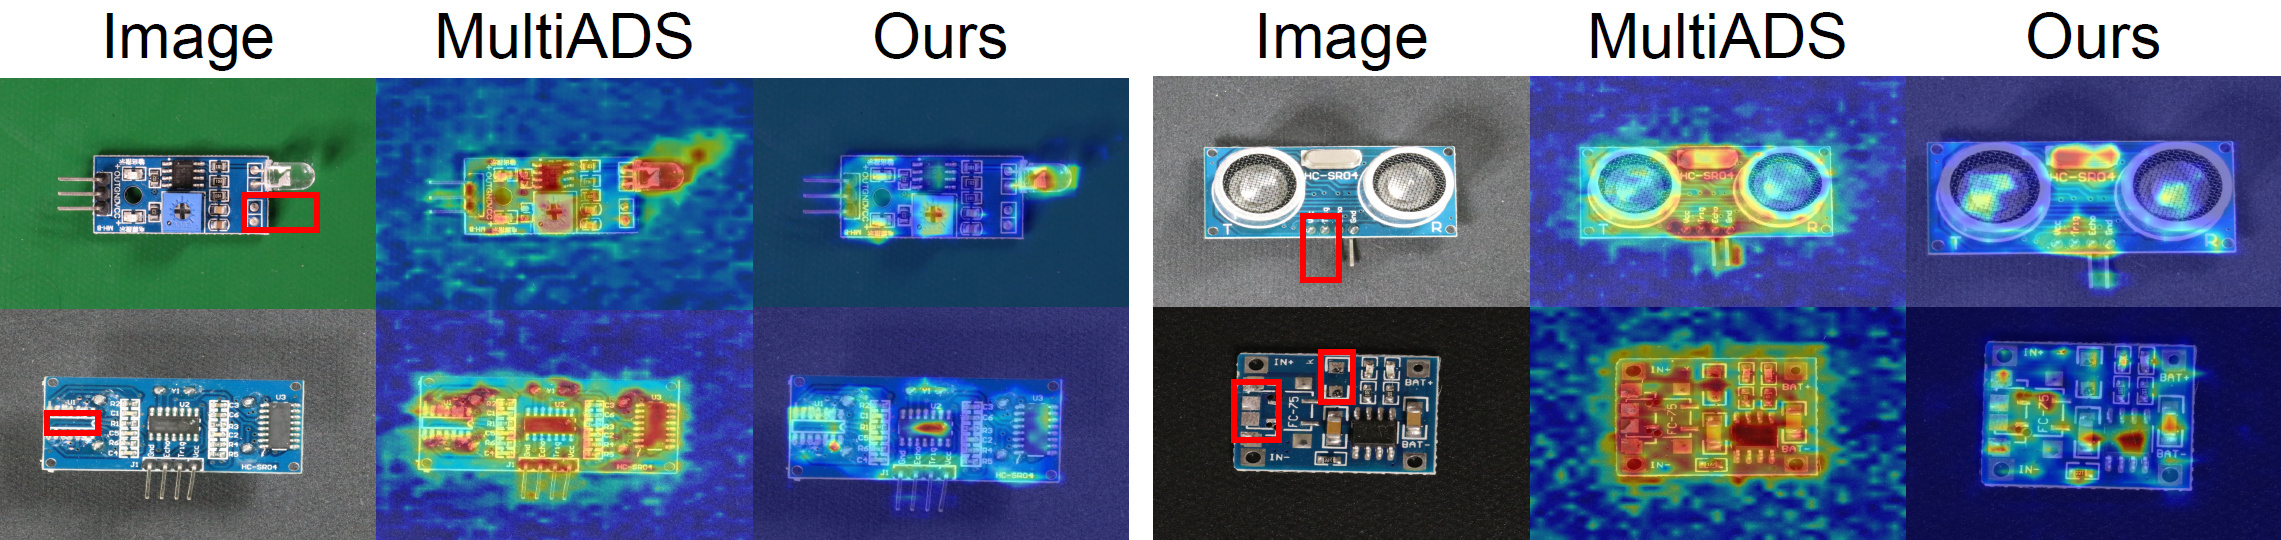
\includegraphics[width=1.0\columnwidth]{imgs/visa-missing.jpg}
  \caption{Anomaly segmentation on VisA for the \emph{missing} defect, a globally-defined anomaly, with MultiADS for comparison. Both methods yield low-confidence, incomplete maps.}
  \label{fig:visa-visual-bad}
\end{figure}
GenAU excels at visually salient anomalies (distinct texture or color deviations), where strong local cues align with the defect-token anchors. Segmentation degrades for globally-defined or logical anomalies (e.g., \textit{missing} or \textit{misplaced} components; Figure~\ref{fig:visa-visual-bad}), which look normal at the patch level and, in the zero-shot setting, give no prior on expected placement; few-shot or domain priors could help.

\subsection{Challenges in Defect-Type Classification}
Fine-grained classification exposes the limits of the VLM's pre-trained knowledge: the same label varies widely across objects (a \textit{missing cable} is a conspicuous void, a \textit{missing LED} blends in; cracks range from large openings to fine lines), so generalization is hard when training shows one instance of a defect. Logical defects further require reasoning about expected structure that the model cannot encode without domain knowledge; broader exposure to each defect would help.

\section{Conclusion}
We presented GenAU, an instruction-following VLM architecture for detection, localization, conditional defect-type recognition, and textual analysis. A single checkpoint, trained with reasoning conversations in half of its samples at an unchanged budget, provides competitive cross-dataset detection and localization and supports all four tasks; giving every sample a conversation doubles the budget and lowers detection and localization. Learned-query controls show a localization benefit on VisA, not universal superiority. Logical anomalies, fine-grained types, and verified causal diagnosis remain open challenges.







% The ICLR-only end-of-main-text statements (AI use / Ethics / Reproducibility)
% are NOT inputted: CVPR requires none of them. sec/8_statements.tex is kept on
% disk unused, in case it is wanted for arXiv or for a venue that asks again.

{
    \small
    \bibliographystyle{ieeenat_fullname}
    \bibliography{custom}
}

%%%%%%%%% SUPPLEMENTARY MATERIAL
% CVPR caps the main paper at 8 pages excluding references, and supplementary
% material is uploaded as a SEPARATE PDF. Following the official author kit
% (sec/X_suppl.tex), the appendix is authored in this same document so that
% cross-references resolve in one compile, and the resulting PDF is SPLIT before
% submission: pages 1..N -> the paper, the rest -> the supplementary.
% *** DO NOT UPLOAD THIS PDF UNSPLIT. ***
% Appendix floats keep the "A" prefix (Table A1, Figure A1) so they are never
% confused with the main paper's Table 1 / Figure 1; the counters restart at 1.
\clearpage
\setcounter{page}{1}
\maketitlesupplementary
\renewcommand{\thetable}{A\arabic{table}}
\renewcommand{\thefigure}{A\arabic{figure}}
\setcounter{table}{0}
\setcounter{figure}{0}
\appendix

\section{Datasets}
\label{app:datasets}
Due to space limitations in the main manuscript, we provide here a detailed description of the industrial anomaly detection datasets used in our experiments: MVTec-AD~\cite{Bergmann_2019_CVPR}, VisA~\cite{VisA}, MPDD~\cite{mpdd}, and Real-IAD~\cite{wang2024realiadrealworldmultiviewdataset}. Key dataset statistics, including the number of defect types, object categories, and the proportion of single- and multi-defect images, are summarized in \cref{tab:dataset_summary}. For all datasets, each defect instance is mapped to a unified defect taxonomy as defined in \crefrange{tab:mvtec-mapping1}{tab:real-iad-mapping2}.
MVTec-AD includes common industrial items such as bottles, cables, zippers, and hazelnuts. VisA contains a mixture of everyday products such as chewing gum and macaroni, as well as more complex components like printed circuit boards. MPDD focuses primarily on industrial parts, including metal brackets, tubes, and machined components. Real-IAD contains a broad range of real-world consumer and industrial items such as audio jacks, switches, bottle caps, and plastic toys.

% Overview of Datasets
\begin{table*}
\centering
\setlength{\tabcolsep}{5pt}
\caption[Overview of the datasets used for evaluation.]{Overview of the datasets used for evaluation. The third column lists distinct defects, while the fourth column counts compound defects treated as separate categories.}
\label{tab:dataset_summary}
\begin{tabular}{cccccc}
\toprule
\textbf{Dataset} & \textbf{Objects} & \textbf{\begin{tabular}[c]{@{}c@{}}Unique \\ Defect Types\end{tabular}} & \textbf{\begin{tabular}[c]{@{}c@{}}Defect Types \\ Incl. Combinations\end{tabular}} & \textbf{\begin{tabular}[c]{@{}c@{}}Single Defect \\ Images\end{tabular}} & \textbf{\begin{tabular}[c]{@{}c@{}}Multi Defect \\ Images\end{tabular}} \\
\midrule
MVTec-AD  & 15 & 16 & 38   & 1,200  & 58   \\
VisA      & 12 & 14 & 56   & 923    & 277  \\
MPDD      & 6  & 6  & 7    & 265    & 17   \\
Real-IAD  & 30 & 9  & 9    & 51,329 & 0    \\
\bottomrule
\end{tabular}
\end{table*}

% MVTec Mapping
\begin{table}
\centering
\footnotesize
\caption{Defect taxonomy for the MVTec-AD dataset (Part I).}
\label{tab:mvtec-mapping1}
\begin{tabular}{@{}ccc@{}}
\toprule
\textbf{Product} & \textbf{Original Defect Types} & \textbf{Mapped Defect Types} \\
\midrule

\multirow{3}{*}{Bottle}
 & Broken Large & Broken \\
 & Broken Small & Broken \\
 & Contamination & Contamination \\

\midrule
\multirow{8}{*}{Cable}
 & Bent Wire & Bent \\
 & Cable Swap & Misplaced \\
 & Combined & Combination of Defects \\
 & Cut Inner Insulation & Cut \\
 & Cut Outer Insulation & Cut \\
 & Missing Cable & Missing \\
 & Missing Wire & Missing \\
 & Poke Insulation & Poke \\

\midrule
\multirow{5}{*}{Capsule}
 & Crack & Crack \\
 & Faulty Imprint & Scratch \\
 & Poke & Crack \\
 & Scratch & Scratch \\
 & Squeeze & Deformed \\

\midrule
\multirow{5}{*}{Carpet}
 & Color & Color \\
 & Cut & Tear \\
 & Hole & Hole \\
 & Metal Contamination & Contamination \\
 & Thread & Contamination \\

\midrule
\multirow{4}{*}{Hazelnut}
 & Crack & Crack \\
 & Cut & Cut \\
 & Hole & Hole \\
 & Print & Color \\

\midrule
\multirow{5}{*}{Grid}
 & Bent & Bent \\
 & Broken & Broken \\
 & Glue & Contamination \\
 & Metal Contamination & Contamination \\
 & Thread & Contamination \\

\midrule
\multirow{5}{*}{Leather}
 & Color & Color \\
 & Cut & Cut \\
 & Fold & Fold \\
 & Glue & Contamination \\
 & Poke & Poke \\

\midrule
\multirow{4}{*}{Metal Nut}
 & Bent & Bent \\
 & Color & Color \\
 & Flip & Misplaced \\
 & Scratch & Scratch \\

\midrule
\multirow{7}{*}{Pill}
 & Color & Color \\
 & Combined & Combination of Defects \\
 & Contamination & Contamination \\
 & Crack & Crack \\
 & Faulty Imprint & Scratch \\
 & Pill Type & Color \\
 & Scratch & Scratch \\

\midrule
\multirow{5}{*}{Screw}
 & Manipulated Front & Bent Head / Broken Tip \\
 & Scratch Head & Damaged \\
 & Scratch Neck & Damaged \\
 & Thread Side & Damaged \\
 & Thread Top & Damaged \\

\bottomrule
\end{tabular}
\end{table}

\begin{table}
\centering
\footnotesize
\caption{Defect taxonomy for the MVTec-AD dataset (Part II).}
\label{tab:mvtec-mapping2}
\begin{tabular}{@{}ccc@{}}
\toprule
\textbf{Product} & \textbf{Original Defect Types} & \textbf{Mapped Defect Types} \\
\midrule

\multirow{5}{*}{Tile}
 & Crack & Crack \\
 & Glue Strip & Contamination \\
 & Gray Stroke & Color \\
 & Oil & Contamination \\
 & Rough & Scratch \\

\midrule
\multirow{1}{*}{Toothbrush}
 & Defective & Bent / Contamination / Missing \\

\midrule
\multirow{4}{*}{Transistor}
 & Bent Lead & Bent \\
 & Cut Lead & Broken \\
 & Damaged Case & Damaged \\
 & Misplaced & Misplaced \\

\midrule
\multirow{5}{*}{Wood}
 & Color & Color \\
 & Combined & Combination of Defects \\
 & Hole & Hole \\
 & Liquid & Contamination \\
 & Scratch & Scratch \\

\midrule
\multirow{7}{*}{Zipper}
 & Broken Teeth & Broken \\
 & Combined & Combination of Defects \\
 & Fabric Border & Tear \\
 & Fabric Interior & Tear \\
 & Rough & Contamination \\
 & Split Teeth & Deformed \\
 & Squeezed Teeth & Deformed \\

\bottomrule
\end{tabular}
\end{table}

% VisA Mapping
\begin{table}
\centering
\scriptsize
\renewcommand{\arraystretch}{0.9}
\caption{Defect taxonomy for the VisA dataset (Part I).}
\label{tab:visa-mapping1}
\begin{tabular}{@{}ccc@{}}
\toprule
\textbf{Product} & \textbf{Original Defect Types} & \textbf{Mapped Defect Types} \\
\midrule

\multirow{8}{*}{Candle}
 & Chunk of Wax Missing & Hole \\
 & Damaged Corner of Packaging & Damaged \\
 & Different Colour Spot & Color \\
 & Extra Wax in the Candle & Contamination \\
 & Foreign Particals on the Candle & Color \\
 & Wax Melded out of the Candle & Melded \\
 & Weird Candle Wick & Weird Wick \\
 & Combined & Combination of Defects \\

\midrule
\multirow{6}{*}{Capsules}
 & Bubble & Bubble \\
 & Discolor & Color \\
 & Scratch & Scratch \\
 & Leak & Contamination \\
 & Misshape & Deformed \\
 & Combined & Combination of Defects \\

\midrule
\multirow{9}{*}{Cashew}
 & Burnt & Color \\
 & Corner or Edge Breakage & Broken \\
 & Different Colour Spot & Color \\
 & Middle Breakage & Broken \\
 & Same Colour Spot & Color \\
 & Small Holes & Hole \\
 & Small Scratches & Scratch \\
 & Stuck Together & Misplaced \\
 & Combined & Combination of Defects \\

\midrule
\multirow{6}{*}{Chewinggum}
 & Chunk of Gum Missing & Broken \\
 & Corner Missing & Broken \\
 & Scratches & Scratch \\
 & Similar Colour Spot & Color \\
 & Small Cracks & Crack \\
 & Combined & Combination of Defects \\

\midrule
\multirow{8}{*}{Fryum}
 & Burnt & Color \\
 & Corner or Edge Breakage & Broken \\
 & Different Colour Spot & Color \\
 & Fryum Stuck Together & Misplaced \\
 & Middle Breakage & Broken \\
 & Similar Colour Spot & Color \\
 & Small Scratches & Scratch \\
 & Combined & Combination of Defects \\

\bottomrule
\end{tabular}
\end{table}

\begin{table}
\centering
\scriptsize
\renewcommand{\arraystretch}{0.9}
\caption{Defect taxonomy for the VisA dataset (Part II).}
\label{tab:visa-mapping2}
\begin{tabular}{@{}ccc@{}}
\toprule
\textbf{Product} & \textbf{Original Defect Types} & \textbf{Mapped Defect Types} \\
\midrule

\multirow{7}{*}{Macaroni1}
 & Chip Around Edge and Corner & Broken \\
 & Different Colour Spot & Color \\
 & Similar Colour Spot & Color \\
 & Small Cracks & Crack \\
 & Middle Breakage & Hole \\
 & Small Scratches & Scratch \\
 & Combined & Combination of Defects \\

\midrule

\multirow{7}{*}{Macaroni2}
 & Breakage down the Middle & Hole \\
 & Color Spot Similar to the Object & Color \\
 & Different Color Spot & Color \\
 & Small Chip Around Edge & Broken \\
 & Small Cracks & Crack \\
 & Small Scratches & Scratches \\
 & Combined & Combination of Defects \\

\midrule
\multirow{5}{*}{pcb1}
 & Bent & Bent \\
 & Melt & Contamination \\
 & Missing & Missing \\
 & Scratch & Scratch \\
 & Combined & Combination of Defects \\

\midrule
\multirow{5}{*}{pcb2}
 & Bent & Bent \\
 & Melt & Contamination \\
 & Missing & Missing \\
 & Scratch & Scratch \\
 & Combined & Combination of Defects \\

\midrule
\multirow{5}{*}{pcb3}
 & Bent & Bent \\
 & Melt & Contamination \\
 & Missing & Missing \\
 & Scratch & Scratch \\
 & Combined & Combination of Defects \\

\midrule
\multirow{8}{*}{pcb4}
 & Burnt & Contamination \\
 & Scratch & Scratch \\
 & Damage & Damaged \\
 & Dirt & Contamination \\
 & Extra & Contamination \\
 & Missing & Missing \\
 & Wrong Place & Contamination \\
 & Combined & Combination of Defects \\

\midrule
\multirow{8}{*}{Pipe Fryum}
 & Burnt & Color \\
 & Corner and Edge Breakage & Broken \\
 & Different Colour Spot & Color \\
 & Similar Colour Spot & Color \\
 & Small Scratches & Scratch \\
 & Stuck Together & Misplaced \\
 & Small Cracks & Crack \\
 & Combined & Combination of Defects \\

\bottomrule
\end{tabular}
\end{table}

% MPDD Mapping
\begin{table}
\centering
\caption{Defect taxonomy for the MPDD dataset.}
\footnotesize
\label{tab:mpdd-mapping}
\begin{tabular}{@{}ccc@{}}
\toprule
\textbf{Product} & \textbf{Original Defects Types}                                                 & \textbf{Mapped Defect Types}                                           \\ \midrule
Bracket Black    & \begin{tabular}[c]{@{}c@{}}Hole\\ Scratch\end{tabular}                           & \begin{tabular}[c]{@{}c@{}}Hole\\ Scratch\end{tabular}                 \\ \midrule
Bracket Brown    & \begin{tabular}[c]{@{}c@{}}Bend and Parts Mismatch\\ Parts Mismatch\end{tabular} & \begin{tabular}[c]{@{}c@{}}Bent and Misplaced\\ Misplaced\end{tabular} \\ \midrule
Bracket White    & \begin{tabular}[c]{@{}c@{}}Defective Painting\\ Scratches\end{tabular}           & \begin{tabular}[c]{@{}c@{}}Contamination\\ Scratch\end{tabular}        \\ \midrule
Connector        & Parts Mismatch                                                                   & Missing                                                                \\ \midrule
Metal Plate      & \begin{tabular}[c]{@{}c@{}}Major Rust\\ Total Rust\\ Scratch\end{tabular}        & \begin{tabular}[c]{@{}c@{}}Color\\ Color\\ Scratch\end{tabular}        \\ \midrule
Tubes            & Anomalous                                                                        & Deformed                                                               \\ \bottomrule
\end{tabular}
\end{table}

% Real-IAD Mapping
\begin{table}
\centering
\footnotesize
\renewcommand{\arraystretch}{0.7}
\caption{Defect taxonomy for the Real-IAD dataset (Part I).}
\label{tab:real-iad-mapping1}
\begin{tabular}{@{}ccc@{}}
\toprule
\textbf{Product} & \textbf{Original Defect Types} & \textbf{Mapped Defect Types} \\
\midrule

\multirow{4}{*}{Audiojack}
 & Contamination & Color \\
 & Missing Parts & Broken \\
 & Deformation & Bent \\
 & Scratch & Scratch \\

\midrule
\multirow{4}{*}{Bottle Cap}
 & Contamination & Color \\
 & Missing Parts & Broken \\
 & Scratch & Scratch \\
 & Pit & Hole \\

\midrule
\multirow{4}{*}{Button Battery}
 & Scratch & Scratch \\
 & Abrasion & Abrasion \\
 & Contamination & Color \\
 & Pit & Color \\

\midrule
\multirow{4}{*}{End Cap}
 & Damage & Broken \\
 & Missing Parts & Broken \\
 & Contamination & Color \\
 & Scratch & Scratch \\

\midrule
\multirow{4}{*}{Eraser}
 & Contamination & Color \\
 & Scratch & Scratch \\
 & Pit & Hole \\
 & Missing Parts & Broken \\

\midrule
\multirow{4}{*}{Fire Hood}
 & Pit & Hole \\
 & Contamination & Color \\
 & Missing Parts & Broken \\
 & Scratch & Scratch \\

\midrule
\multirow{3}{*}{Mint}
 & Missing Parts & Broken \\
 & Foreign Objects & Contamination \\
 & Contamination & Contamination \\

\midrule
\multirow{3}{*}{Mounts}
 & Missing Parts & Broken \\
 & Contamination & Color \\
 & Pit & Hole \\

\midrule
\multirow{4}{*}{PCB}
 & Missing Parts & Missing \\
 & Scratch & Scratch \\
 & Foreign Objects & Contamination \\
 & Contamination & Contamination \\

\midrule
\multirow{4}{*}{Phone Battery}
 & Damage & Broken \\
 & Pit & Hole \\
 & Scratch & Scratch \\
 & Contamination & Contamination \\

\midrule
\multirow{4}{*}{Plastic Nut}
 & Pit & Hole \\
 & Scratch & Scratch \\
 & Contamination & Contamination \\
 & Damage & Broken \\

\midrule
\multirow{4}{*}{Plastic Plug}
 & Missing Parts & Broken \\
 & Scratch & Scratch \\
 & Pit & Hole \\
 & Contamination & Contamination \\

\midrule
\multirow{3}{*}{Porcelain Doll}
 & Scratch & Scratch \\
 & Abrasion & Abrasion \\
 & Contamination & Color \\

\bottomrule
\end{tabular}
\end{table}

\begin{table}
\centering
\footnotesize
\renewcommand{\arraystretch}{0.7}
\caption{Defect taxonomy for the Real-IAD dataset (Part II).}
\label{tab:real-iad-mapping2}
\begin{tabular}{@{}ccc@{}}
\toprule
\textbf{Product} & \textbf{Original Defect Types} & \textbf{Mapped Defect Types} \\
\midrule

\multirow{4}{*}{Regulator}
 & Contamination & Color \\
 & Missing Parts & Broken \\
 & Scratch & Scratch \\
 & Pit & Hole \\

\midrule
\multirow{3}{*}{Rolled Strip Base}
 & Pit & Hole \\
 & Missing Parts & Broken \\
 & Contamination & Color \\

\midrule
\multirow{3}{*}{SIM Card Set}
 & Scratch & Scratch \\
 & Abrasion & Scratch \\
 & Contamination & Contamination \\

\midrule
\multirow{3}{*}{Switch}
 & Missing Parts & Broken \\
 & Contamination & Contamination \\
 & Scratch & Scratch \\

\midrule
\multirow{4}{*}{Tape}
 & Scratch & Scratch \\
 & Missing Parts & Broken \\
 & Damage & Broken \\
 & Contamination & Color \\

\midrule
\multirow{3}{*}{Terminalblock}
 & Pit & Hole \\
 & Missing Parts & Broken \\
 & Contamination & Color \\

\midrule
\multirow{3}{*}{Toothbrush}
 & Missing Parts & Broken \\
 & Contamination & Contamination \\
 & Abrasion & Deformed \\

\midrule
\multirow{4}{*}{Toy}
 & Scratch & Scratch \\
 & Contamination & Color \\
 & Missing Parts & Broken \\
 & Pit & Hole \\

\midrule
\multirow{4}{*}{Toy Brick}
 & Contamination & Color \\
 & Pit & Hole \\
 & Missing Parts & Broken \\
 & Scratch & Scratch \\

\midrule
\multirow{3}{*}{Transistor1}
 & Missing Parts & Broken \\
 & Deformation & Bent \\
 & Contamination & Contamination \\

\midrule
\multirow{4}{*}{U Block}
 & Missing Parts & Broken \\
 & Scratch & Scratch \\
 & Abrasion & Scratch \\
 & Contamination & Color \\

\midrule
\multirow{4}{*}{USB}
 & Scratch & Scratch \\
 & Deformation & Bent \\
 & Contamination & Color \\
 & Missing Parts & Broken \\

\midrule
\multirow{4}{*}{USB Adaptor}
 & Contamination & Color \\
 & Scratch & Scratch \\
 & Abrasion & Scratch \\
 & Pit & Broken \\

\midrule
\multirow{4}{*}{Vcpill}
 & Contamination & Color \\
 & Scratch & Scratch \\
 & Missing Parts & Broken \\
 & Pit & Broken \\

\midrule
\multirow{4}{*}{Wooden Beads}
 & Scratch & Scratch \\
 & Contamination & Color \\
 & Pit & Hole \\
 & Missing Parts & Broken \\

\midrule
\multirow{4}{*}{Woodstick}
 & Contamination & Color \\
 & Scratch & Scratch \\
 & Pit & Hole \\
 & Missing Parts & Broken \\

\midrule
\multirow{4}{*}{Zipper}
 & Missing Parts & Broken \\
 & Damage & Broken \\
 & Deformation & Deformed \\
 & Contamination & Color \\

\bottomrule
\end{tabular}
\end{table}

\section{Implementation Details}
\label{app:impl}
We build GenAU on the LLaVA-OneVision family~\cite{li2025llavaonevision}, which couples a Qwen2 language backbone with a SigLIP-so400m-patch14-384 vision encoder, and report the 0.5B and 7B scales. High-resolution inputs use the AnyRes scheme (\texttt{anyres\_max\_9}) with an image grid of up to $6\times6$ tiles of $384$ pixels, in addition to a global low-resolution view. For the segmentation readout we take patch features from four vision-encoder stages (layers $6$, $12$, $18$, and the final layer) and equip each stage with its own linear projection into the decoder hidden space.

\paragraph{Trainable parameters.}
The vision encoder is frozen; the cross-modal projector is trained with a learning rate of $10^{-4}$. The LLM is adapted with rank-stabilized LoRA (rank $r=16$, $\alpha=32$, dropout $0$). The token-embedding table and language-modeling head are fully fine-tuned to integrate the two added segmentation tokens \texttt{[SEG\_normal]} and \texttt{[SEG\_defect]}, and the four segmentation projectors together with the decoder layer-norms are trainable.

\paragraph{Optimization.}
Training runs for a single epoch with an effective batch size of $32$ (per-device batch $1$, gradient accumulation $4$, across $8$ GPUs with DeepSpeed ZeRO-3), a learning rate of $10^{-4}$ with cosine decay, a warmup ratio of $0.03$, and no weight decay. The segmentation objective sums, over the four stages, a focal term on the upsampled logits, a Tversky term ($\alpha=0.3$, $\beta=0.7$) on the defect channel that up-weights false negatives, and a Dice term on the complementary normal channel; the text-to-segmentation weight is $\lambda=1$.

\paragraph{High-resolution readout and image-level fusion.}
At inference the high-resolution and global-view anomaly maps are fused per stage as $\mathbf{A}=(1-\beta)\,\mathbf{A}^{\mathrm{g}}+\beta\,\mathbf{A}^{\mathrm{hi}}$ with $\beta=0.25$ and a similarity temperature of $20$. The image-level score fuses the spatial maximum of $\mathbf{A}$ with the decoder's normal/defect log-odds, averaged over eight phrasings of the yes/no question (the templates used by the VisA and MPDD benchmarks; the image prefix is encoded once and its cache reused for each phrasing). The two are each $z$-score standardized with statistics estimated once on the MVTec calibration split and averaged with equal weights; the standardization is frozen and shared across target datasets, so no target-domain labels are used. If a generated answer omits the two segmentation tokens, they are appended to it and their hidden states are read with one additional forward pass, so every test image receives a defect map.

\section{Training Data Construction}
\label{app:data}
The segmentation instruction data for the reported cross-dataset experiments use MVTec-AD~\cite{Bergmann_2019_CVPR} as the source benchmark. We retain its images and masks and add instruction--response pairs. Each sample consists of an image, mask, instruction, and response; the instruction asks whether the named object contains an anomaly and requests localization, e.g.\ \texttt{``Is there any anomaly on the \{object\}? If yes, segment it.''}

The response describes the anomaly in natural language and terminates with the two segmentation tokens \texttt{[SEG\_defect]} and \texttt{[SEG\_normal]}, from which the localization read-out is taken; for a normal image it instead states that no anomaly is present. An example response is:

\textit{``Yes, there is an anomaly on the capsule. Specifically, there is a dent on the orange side, affecting the clarity and smoothness of the numeral `0' in the printed number `500.' [SEG\_defect] [SEG\_normal]''}

\paragraph{Reasoning conversations.} For $863$ of the $1{,}725$ training images (drawn at random), the single exchange is replaced by a multi-turn conversation about the same image from the instruction data of Anomaly-OV~\cite{xu2025towards}: an image description, the segmentation request above (answered with the two segmentation tokens), and three to nine follow-up questions on the defect's appearance, significance, likely cause, and prevention. The remaining $862$ images keep the single segmentation exchange. Every image appears exactly once, so the number of samples and optimization steps ($53$ at batch size $32$) matches segmentation-only training; adding the conversations as extra samples instead doubles the steps, to which this recipe is sensitive (Table~\ref{tab:ablations_main}).

\section{Defect Taxonomy}
\label{app:taxonomy}
Industrial AD datasets often define highly specific defect categories, which can lead to overfitting and inconsistent label usage~\cite{mokhtar2025detectclassifyactcategorizing}. To improve generalization, we map product-specific labels to a unified, coarser taxonomy, following MultiADS~\cite{sadikaj2025multiadsdefectawaresupervisionmultitype}: e.g., \textit{liquid} and \textit{metal contamination} are merged into \textit{contamination}, and \textit{broken large}/\textit{broken small} are unified as \textit{broken}. The taxonomy is defined per object, so the candidate defect set differs across product categories. This reclassification promotes abstraction over product-specific anomalies and mitigates label imbalance, and it does not affect comparisons with prior binary-detection methods, whose metrics are independent of class granularity. The complete per-object mapping for all four datasets is given in \crefrange{tab:mvtec-mapping1}{tab:real-iad-mapping2}.

\section{Evaluation Protocol}
\label{app:eval}
All models are evaluated under single-image inference: only the query image is available at test time, with no reference, support, or exemplar images. GenAU is fine-tuned on the MVTec-AD test split (the only MVTec split carrying anomaly masks and defect-type labels, as the train split contains normal images only) and evaluated, without retraining, on the test splits of VisA, MPDD, and Real-IAD; MVTec thus serves purely as the source domain and is disjoint from all evaluation targets, so no test-time information leaks into the reported numbers. For Real-IAD we use the single-view setting.

\paragraph{Unified inspection prompt.}
For binary detection and segmentation, the instruction names the object category and requests an anomaly decision and its localization. The model is trained to follow its answer with both segmentation tokens. If generation omits them, they are appended and read in an extra forward pass. Thus both anchors are always \emph{available}, not necessarily generated spontaneously, and all evaluated images receive maps.

\paragraph{Product-conditioned multi-type detection.}
The reported multi-type table evaluates forced-choice recognition on known-anomalous images: $916$ mapped VisA images and all $282$ MPDD anomalous images. The instruction explicitly states anomaly presence, lists the target object's coarse candidate labels, and requests one option; normal is excluded from both the options and scoring. Images whose original label has no coarse mapping are excluded before evaluation. A compound defect may map to one \emph{combined} class; this is not independent multi-label recovery. The supplied object vocabulary is target-domain metadata, not a prediction of the valid vocabulary.

The parser lowercases the response, replaces underscores with spaces, and searches for candidate labels and their mapped fine-label synonyms. The earliest matching substring wins; no match returns \texttt{none}, counted as an incorrect prediction. Weighted precision, recall, and F1 are computed over the pooled images with class-support weights and zero scores for undefined divisions, rather than averaging per-object F1. Every image in each mapped subset has an answer in the reported runs. This protocol does not measure normal-image false positives; the binary task evaluates those separately.

\paragraph{Single-checkpoint evaluation.}
Every task uses the checkpoint of Table~\ref{tab:binary}, without weight changes. Detection and segmentation use their inspection prompt; type recognition uses the forced-choice prompt; VisA-D\&R uses its conversational questions. On VisA-D\&R, GenAU-7B's SBERT similarity to the reference answers is $0.579$ (low-level) and $0.664$ (complex), against $0.590$/$0.576$ for the segmentation-only checkpoint with a frozen projector and $0.571$/$0.666$ for the full reasoning mix of Table~\ref{tab:ablations_main}; the full mix, however, lowers VisA image-AUROC to $87.0\%$, pixel-AUPRO to $85.8\%$, and type-recognition F1 to $29.0\%$/$69.8\%$ (VisA/MPDD). For GenAU-0.5B the three pairs are $0.554$/$0.635$, $0.564$/$0.560$, and $0.565$/$0.656$.

\section{Additional Ablations}
\label{app:ablation}
Table~\ref{tab:ablations} ablates, on MVTec-AD$\rightarrow$VisA, four training choices of the segmentation-only recipe with a frozen cross-modal projector: the text-to-segmentation loss weight $\lambda$, the number of intermediate vision-encoder stages $m$ supplying the segmentation readout, whether the cross-modal projection to the LLM is trainable, and whether the vision encoder itself is unfrozen. Each row changes a single factor relative to the shaded reference row.

Raising the text-to-segmentation weight to $\lambda=5$ changes little: pixel-AUROC rises by $0.6$, and pixel-AUPRO and image-AUROC each fall by $0.2$ points, so we keep the balanced $\lambda=1$. Reducing the segmentation readout to $m=3$ intermediate stages is also close to neutral (pixel-AUPRO $88.4$ vs.\ $88.7$, image-AUROC $90.7$ vs.\ $90.5$), so the fourth stage adds little. Making the cross-modal projection trainable slightly improves both pixel metrics ($+0.5$ AUROC and AUPRO) but lowers image-AUROC by $0.6$ points; on segmentation-only data the difference is small, and the default recipe trains the projector because, with reasoning conversations in the training data, it recovered localization in our development runs. Finally, unfreezing the vision encoder is markedly harmful, collapsing pixel-AUPRO to $81.8$ and image-AUROC to $75.6$ --- far below every other configuration --- as the encoder over-fits the small fine-tuning set and forgets its general visual features; freezing it is therefore essential.

\begin{table}[h]
\centering
\small
\setlength{\tabcolsep}{3pt}
\caption{Ablation of single training factors on MVTec-AD$\rightarrow$VisA. The shaded row is the segmentation-only GenAU-7B with a frozen projector ($m{=}4$, $\lambda{=}1$, vision encoder frozen); each subsequent row changes one factor. Image columns use the fused score of Table~\ref{tab:binary}. All metrics in \%.}
\label{tab:ablations}
\begin{tabular}{@{}l|cc|cc@{}}
\toprule
 & \multicolumn{2}{c|}{\textbf{Pixel}} & \multicolumn{2}{c}{\textbf{Image}} \\
\cmidrule(lr){2-3}\cmidrule(lr){4-5}
 & AUROC & AUPRO & AUROC & AP \\
\midrule
\rowcolor{gray!20}
segmentation only, frozen projector & 95.1 & 88.7 & 90.5 & 91.9 \\ 
\midrule
\quad $\lambda = 5$            & 95.7 & 88.5 & 90.3 & 91.9 \\ 
\quad $m = 3$ stages          & 94.9 & 88.4 & 90.7 & 92.3 \\ 
\quad projection trainable    & 95.6 & 89.2 & 89.9 & 91.5 \\
\quad vision encoder unfrozen & 94.4 & 81.8 & 75.6 & 79.7 \\
\bottomrule
\end{tabular}
\end{table}

\subsection{Decoder-Conditioned versus Learned-Query Anchors}
\label{app:anchors}
On the segmentation-only recipe with a frozen projector, we replace the two decoder-conditioned anchors with randomly initialized trainable constant queries, keeping the trainable segmentation projection and matched inference. Both arms receive maps for every image; omitted segmentation tokens in the decoder arm are appended before readout. The queries are learned during training, not fixed random vectors at test time.

Table~\ref{tab:anchor_seeds} reports pixel-AUPRO for seeds $42$, $43$, and $44$. Decoder anchors lead on VisA in all three runs, but the $+4.40$-point mean difference is influenced by the learned-query seed-$43$ result of $77.13\%$. On MPDD they lead in two seeds but have a lower mean; on Real-IAD they lead in one. Three seeds characterize training variability, not statistical significance or a guarantee of transfer. The control tests decoder conditioning as a whole, and does not isolate linguistic semantics from image conditioning or optimization effects.

\begin{table}[t]
\centering
\small
\setlength{\tabcolsep}{3pt}
\caption{Matched anchor controls: pixel-AUPRO (\%). Mean rows give mean $\pm$ sample standard deviation across three seeds; $\Delta$ is decoder minus learned-query AUPRO in percentage points.}
\label{tab:anchor_seeds}
\begin{tabular}{@{}llrrr@{}}
\toprule
\textbf{Dataset} & \textbf{Seed} & \textbf{Decoder} & \textbf{Learned} & $\boldsymbol{\Delta}$ \\
\midrule
VisA & 42 & 88.66 & 87.38 & $+1.28$ \\
  & 43 & 87.70 & 77.13 & $+10.57$ \\
  & 44 & 89.32 & 87.99 & $+1.33$ \\
  & Mean & $88.56\pm0.81$ & $84.16\pm6.10$ & $+4.40$ \\
\midrule
MPDD & 42 & 88.91 & 88.73 & $+0.19$ \\
  & 43 & 87.16 & 86.58 & $+0.59$ \\
  & 44 & 87.11 & 89.31 & $-2.19$ \\
  & Mean & $87.73\pm1.02$ & $88.20\pm1.44$ & $-0.47$ \\
\midrule
Real-IAD & 42 & 87.93 & 89.71 & $-1.78$ \\
      & 43 & 86.69 & 82.80 & $+3.89$ \\
      & 44 & 85.38 & 89.53 & $-4.15$ \\
      & Mean & $86.67\pm1.27$ & $87.35\pm3.94$ & $-0.68$ \\
\bottomrule
\end{tabular}
\end{table}

\section{Formal Task Definitions}
\label{app:tasks}
We give the full definitions of the three tasks summarized in Section~\ref{sec:prelims}.

\paragraph{Binary anomaly detection under distribution shift.}
Let $\mathcal{D}_{\text{train}}=\{(\boldsymbol{x}_i,y_i)\}_{i=1}^{N_1}$ and $\mathcal{D}_{\text{target}}=\{(\boldsymbol{x}_i,y_i)\}_{i=N_1+1}^{N_1+N_2}$ be two image--label datasets drawn from different input distributions $\mathcal{P}(\mathcal{X}),\mathcal{P}(\mathcal{X}')$: $\forall i\in\{1,\dots,N_1\}$, $\boldsymbol{x}_i\sim\mathcal{P}(\mathcal{X})$, and $\forall i\in\{N_1+1,\dots,N_1+N_2\}$, $\boldsymbol{x}_i\sim\mathcal{P}(\mathcal{X}')$, where $\mathcal{P}(\mathcal{X})\nsim\mathcal{P}(\mathcal{X}')$. Each image $\boldsymbol{x}\in\mathbb{R}^{H\times W}$ is labeled with $y\in\{0,1\}$ indicating anomaly presence. A binary detector $\hat{f}(\cdot)$ is trained solely on $\mathcal{D}_{\mathrm{train}}$; at test time it is optionally adapted to $\hat{f}'(\cdot)$ using auxiliary target-domain metadata such as a product description. For each $\boldsymbol{x}\in\mathcal{D}_{\mathrm{target}}$, the detector classifies it as normal or anomalous.

\paragraph{Binary anomaly segmentation under distribution shift.}
With $\mathcal{D}_{\text{train}}$ and $\mathcal{D}_{\text{target}}$ as above and $\mathcal{P}(\mathcal{X})\nsim\mathcal{P}(\mathcal{X}')$, each image $\boldsymbol{x}\in\mathbb{R}^{H\times W}$ is paired with a binary mask $\boldsymbol{y}\in\{0,1\}^{H\times W}$ indicating the presence of anomalies at each pixel. The segmentation model $\hat{f}(\cdot)$ is trained solely on $\mathcal{D}_{\mathrm{train}}$ and optionally adapted to $\hat{f}'(\cdot)$ with target-domain metadata. For each pixel of $\boldsymbol{x}\in\mathcal{D}_{\mathrm{target}}$, it classifies the pixel as normal or anomalous.

\paragraph{Conditional defect-type recognition under distribution shift.}
For a known-anomalous target image $\boldsymbol{x}$ of object $o$, the supplied candidate set $C_{\mathrm{target}}(o)$ contains mapped coarse defect labels, including compound classes where defined. The target label is one member $y'\in C_{\mathrm{target}}(o)$, and the model predicts one label through conditional generation and parsing. The target vocabulary mixes labels seen in source training and novel labels; normal images and unmapped defect labels are outside this conditional evaluation. This setting tests cross-dataset type recognition with a supplied vocabulary, not arbitrary multi-label prediction or discovery of the target taxonomy.

\section{Extended Related Work}
\label{app:related}
This expands the related-work overview of the main text.

\paragraph{CLIP-based prompt adaptation for anomaly detection and segmentation.}
Recent advances in industrial anomaly detection/segmentation have largely built upon CLIP due to its strong zero-shot transfer ability, although CLIP was not originally designed for industrial inspection. A major line of work adapts CLIP to industrial AD through normal/abnormal prompts, learnable prompt tokens, or improved visual--text alignment. WinCLIP~\cite{jeong2023winclip} introduces normal and abnormal textual prompts together with window-based feature aggregation for zero-shot anomaly detection. AnomalyCLIP~\cite{zhou2024anomalyclip} learns object-agnostic prompts to capture generic semantics of normality and abnormality, while PromptAD~\cite{Li_2024_WACV} improves state discrimination by adding learnable prefix and suffix tokens. AdaCLIP~\cite{Cao_2024} further combines static and dynamic learnable prompts for adaptive inference across object categories. Beyond prompt learning, CLIP-based methods have been extended to localization and segmentation by improving patch-level alignment or incorporating external modules. APRIL-GAN~\cite{chen2023zero}, AnoCLIP~\cite{deng2024}, and SimCLIP~\cite{simclip} enhance cross-modal alignment for pixel-level anomaly mapping, while CLIP-SAM~\cite{li2024clipsamclipsamcollaboration} and FiLo~\cite{gu2024filozeroshotanomalydetection} combine CLIP with external segmentation or grounding models, and MultiADS~\cite{sadikaj2025multiadsdefectawaresupervisionmultitype} introduces defect-aware textual supervision for multi-type anomaly detection. Other approaches, such as MuSc~\cite{li2024musczeroshotindustrialanomaly}, MAEDAY~\cite{schwartz2024maeday}, and Aota et al.~\cite{aota2023zero}, rely on patch comparison, feature uniformity, or reconstruction difficulty. Despite their effectiveness, these methods largely depend on CLIP-style embedding comparison, external localization modules, or non-generative anomaly scoring, making them less suited for unified defect reasoning and analysis.

\paragraph{Autoregressive VLMs for anomaly detection and reasoning.}
Autoregressive VLMs provide a different paradigm for anomaly understanding by enabling open-ended visual reasoning and instruction-following interaction. Instead of comparing an image embedding with a fixed set of CLIP prompts, they can generate textual descriptions, answer inspection questions, and reason over defect attributes in natural language. AnomalyGPT~\cite{gu2023anomalygptdetectingindustrialanomalies} is an early effort: it introduces an instruction-following VLM for industrial anomaly reasoning and lets users query the model about abnormal regions, but it relies on an external CLIP-based anomaly map combined with the input image and provided to the language model, so the VLM mainly serves as a reasoning interface on top of a separately generated map. More recently, Anomaly-OV~\cite{xu2025towards} specializes multimodal large language models for zero-shot anomaly detection and defect reasoning via Anomaly-Instruct-125k, a large-scale visual instruction-tuning dataset for anomaly-centric understanding; however, it mainly targets image-level detection and explanatory reasoning, while pixel-level segmentation is not explicitly grounded in the autoregressive decoding process.

\section{Detailed Evaluation Metrics}
\label{app:metrics}
We adopt standard metrics for each task. For image-level anomaly detection, we report the Area Under the Receiver Operating Characteristic Curve (AUROC) and Average Precision (AP). For segmentation, we report the pixel-level AUROC and the Area Under the Per-Region Overlap (AUPRO). For multi-type anomaly detection, we use weighted Precision, Recall, and F1-score to account for the strong class imbalance across defect categories. For defect reasoning, we follow the VisA-D\&R protocol~\cite{xu2025towards} and report a GPT-Score in which GPT-4o rates each response on a $1$--$10$ scale, separately for low-level (perception) and complex (causal-reasoning) questions.
The local reference-similarity evaluation uses $1{,}000$ VisA-D\&R entries: turn $0$ is low-level perception and later turns are complex reasoning. SBERT uses \texttt{all-MiniLM-L6-v2} cosine similarity, with low-level/complex scores $0.579$/$0.664$ and overall $0.643$. These metrics quantify reference agreement, not verified root causes. All baselines in Table~\ref{tab:reasoning} are generated and scored with this same pipeline; published scores are not used.

\section{Qualitative Results}
\label{app:qualitative}
In this section, we provide additional visualizations of anomaly segmentation results together with example text responses generated by the model. We present eight samples from diverse products, including tubes (\cref{fig:tubes}) from MPDD, capsules (\cref{fig:capsules}) and pipe fryum (\cref{fig:pipe-fryum}) from VisA, and mounts (\cref{fig:mounts}) and rolled strip base (\cref{fig:rolled_strip_base}) from Real-IAD.

For the tubes, the model precisely identifies the deformed section and preserves clean boundaries, introducing almost no spurious activations elsewhere in the images. A similar pattern holds for the capsules, where the model distinguishes among different defect manifestations, correctly localizing internal bubbles, subtle surface scratches, and areas showing signs of leakage. For the pipe fryum, the model maintains high confidence across several defect types, producing focused masks for color specks, fine scratches, and fractured edges, and doing so consistently across varying shapes and orientations.
On the Real-IAD mounts, the model is able to localize defects but introduces substantial prediction noise. It also occasionally assigns elevated similarity scores to background regions, even when those regions are uniform black and contain no structural cues. For the rolled strip base, the model effectively captures the primary defect, although the anomaly map exhibits considerable background noise and incorrectly attributes medium similarity scores to structural features such as the central diagonal ribs, despite these regions being non-defective.

In \cref{fig:text}, we show examples of how the model classifies defects across different products together with the corresponding segmentation masks. For the cashew sample, it correctly notes the presence of a dark region on the surface, corresponding to a \textit{color} defect. For the pipe fryum, it identifies that several pieces are touching and classifies the issue as \textit{misplaced}. For the PCB, it detects the \textit{bent} defect by recognizing the curved pins. Combined with the segmentation masks, these textual explanations provide detailed and actionable information that can support process optimization.

\begin{figure*}
  \centering
  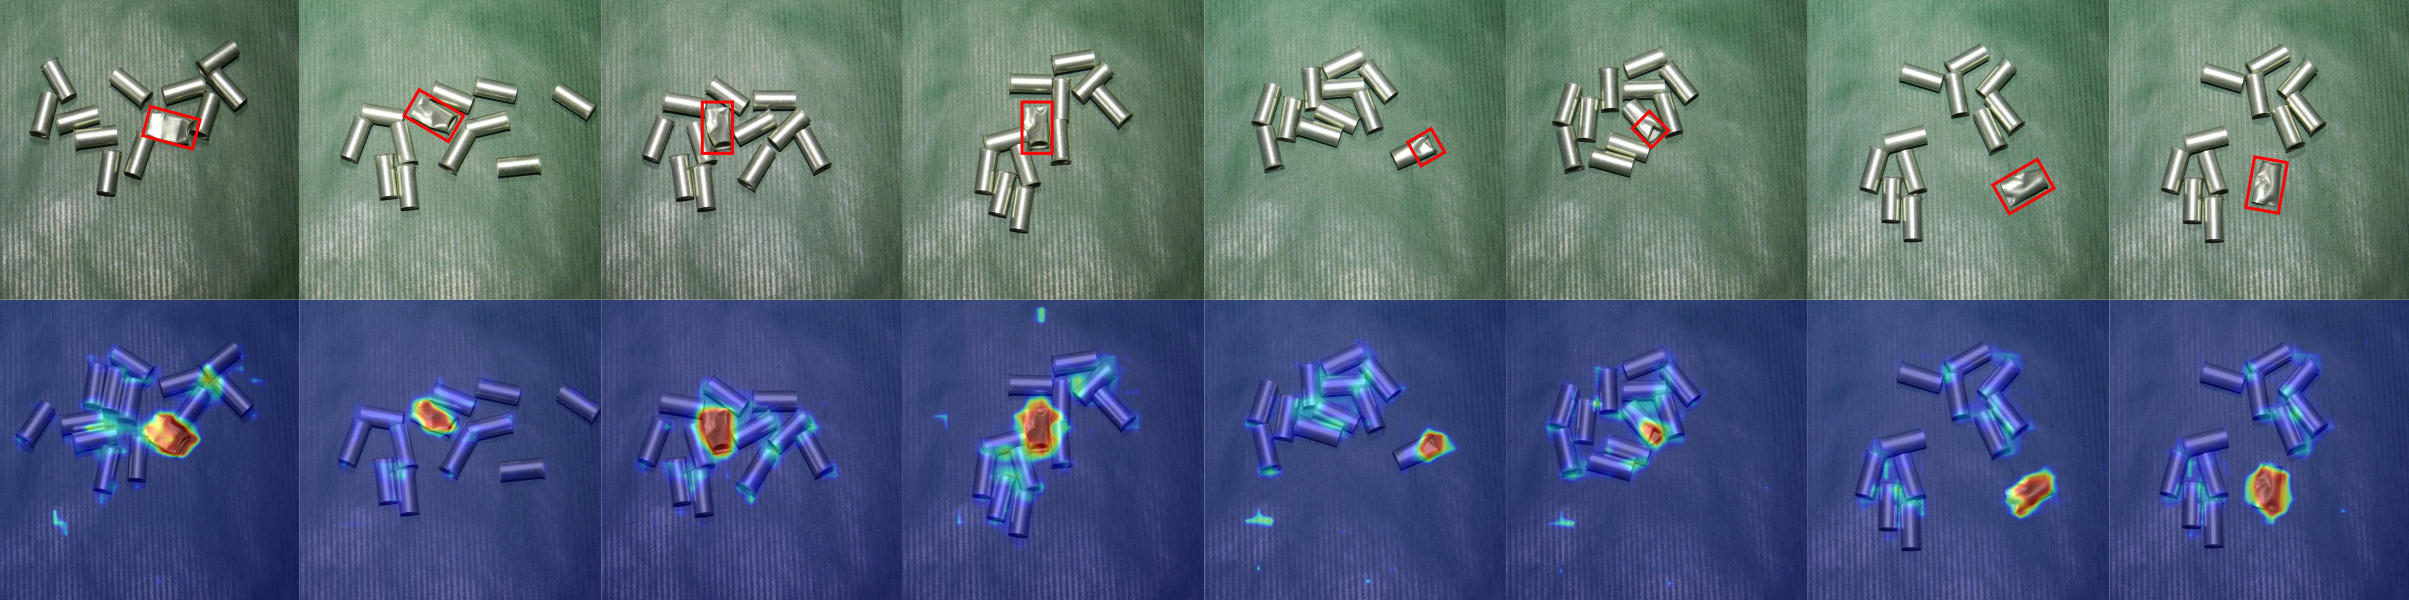
\includegraphics[width=\textwidth]{imgs/tubes.jpg}
  \caption{This visualization showcases the tube product from the MPDD dataset. The first row represents the input with the anomaly highlighted. The second row presents the segmentation results
from our model.}
   \label{fig:tubes}
\end{figure*}

\begin{figure*}
  \centering
  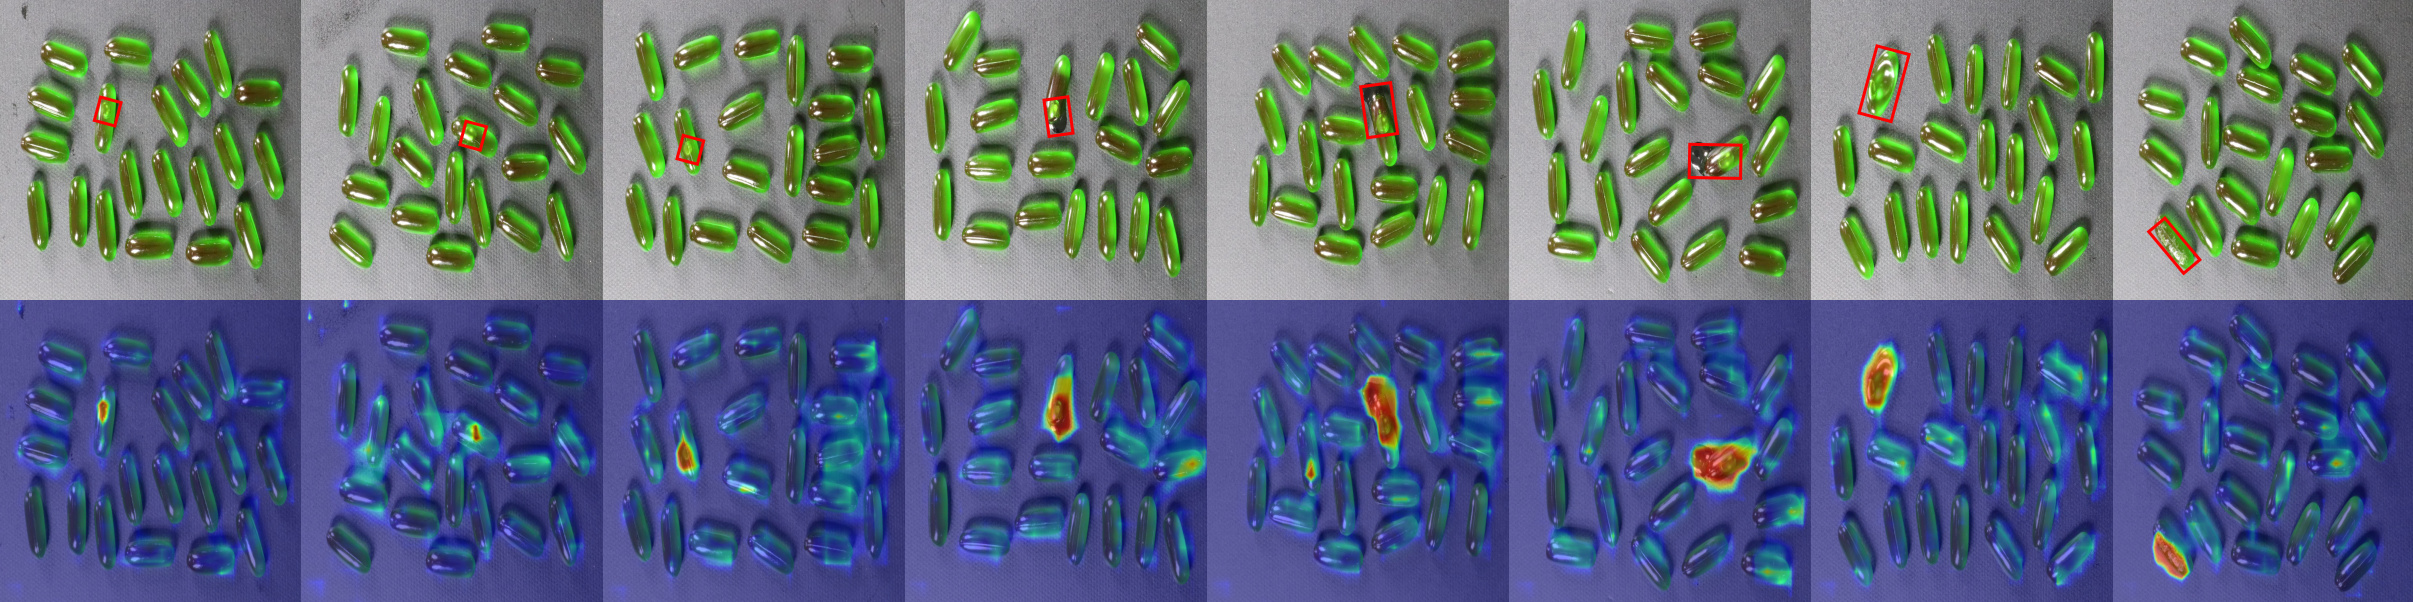
\includegraphics[width=\textwidth]{imgs/capsules.jpg}
  \caption{This visualization showcases the capsule product from the VisA dataset. The first row represents the input with the anomaly highlighted. The second row presents the segmentation results
from our model.}
   \label{fig:capsules}
\end{figure*}

\begin{figure*}
  \centering
  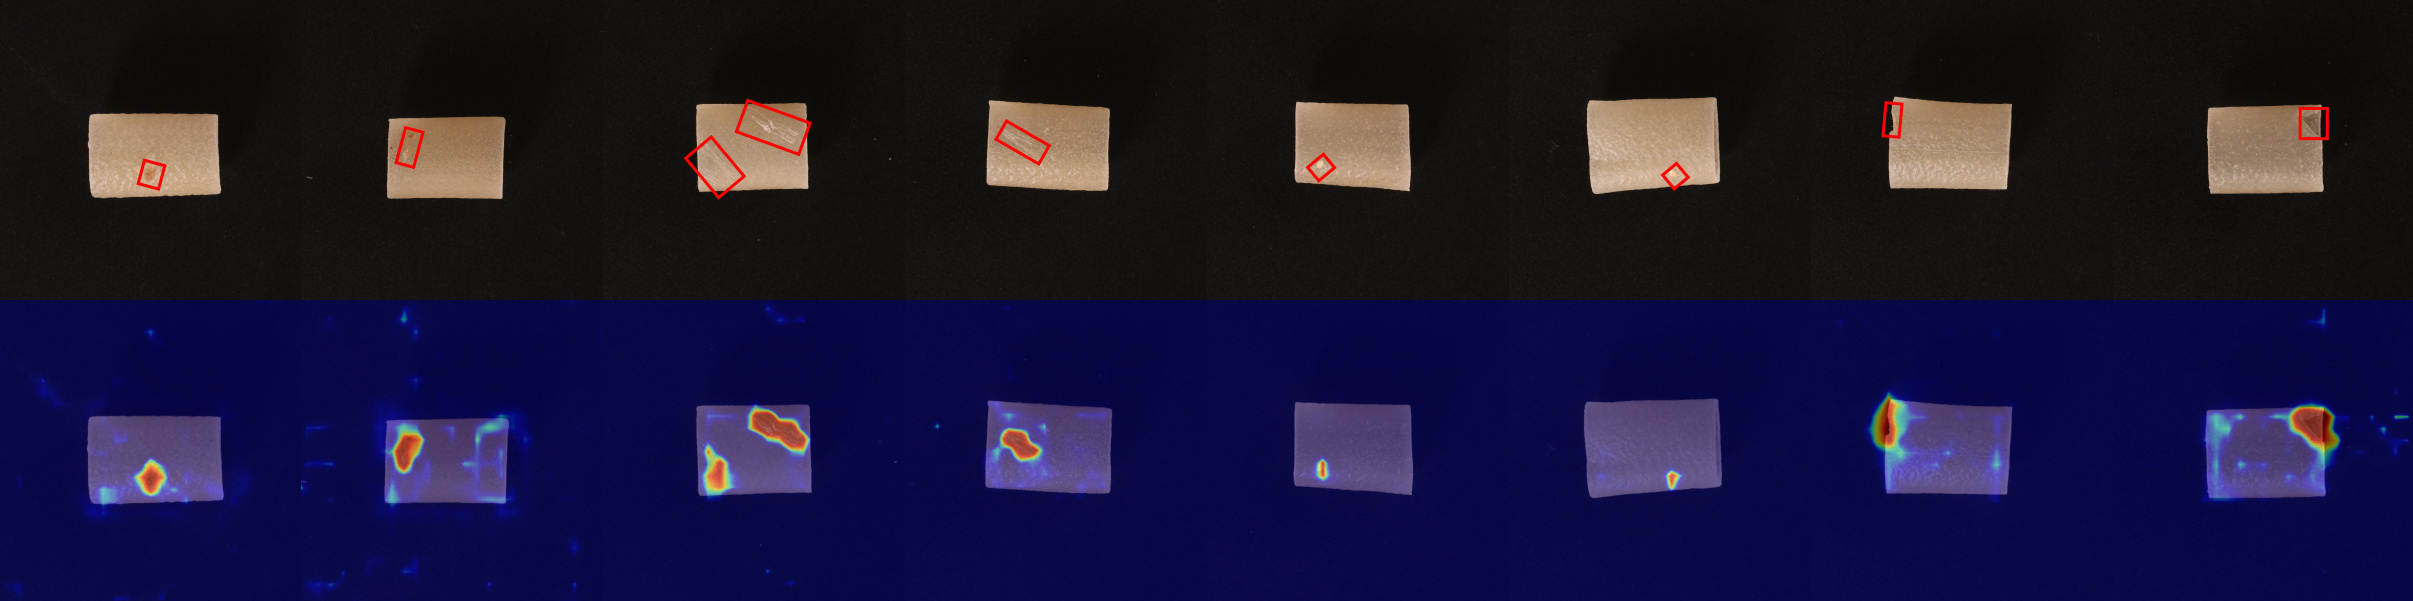
\includegraphics[width=\textwidth]{imgs/pipe-fryum.jpg}
  \caption{This visualization showcases the pipe fryum product from the VisA dataset. The first row represents the input with the anomaly highlighted. The second row presents the segmentation results
from our model.}
   \label{fig:pipe-fryum}
\end{figure*}

\begin{figure*}
  \centering
  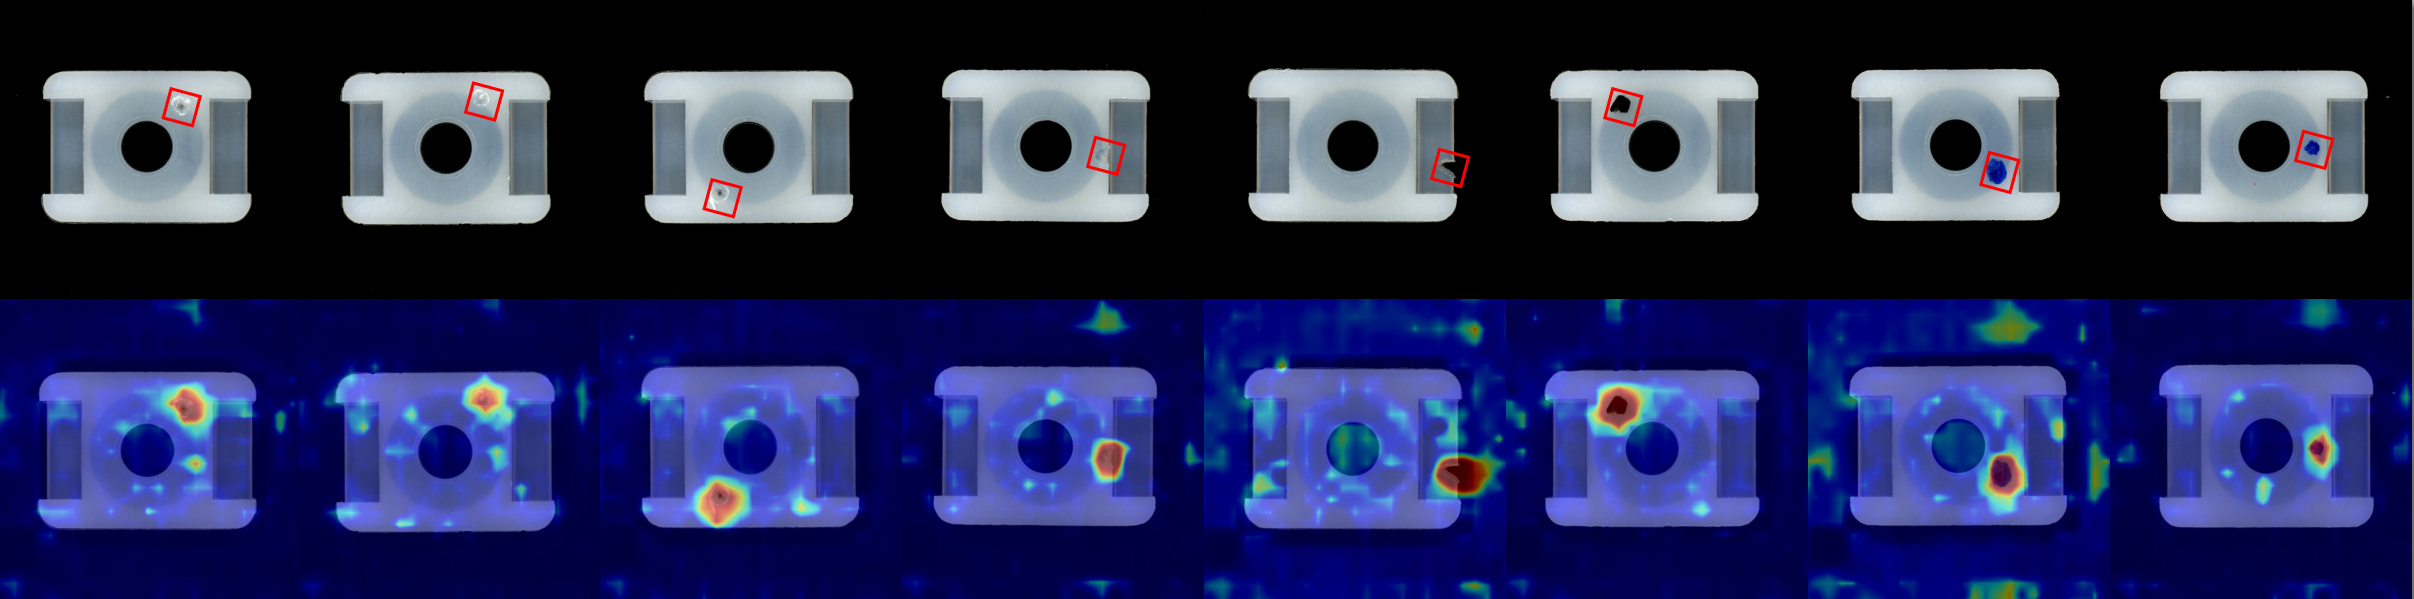
\includegraphics[width=\textwidth]{imgs/mounts.jpg}
  \caption{This visualization showcases the mount product from the Real-IAD dataset. The first row represents the input with the anomaly highlighted. The second row presents the segmentation results
from our model.}
   \label{fig:mounts}
\end{figure*}

\begin{figure*}
  \centering
  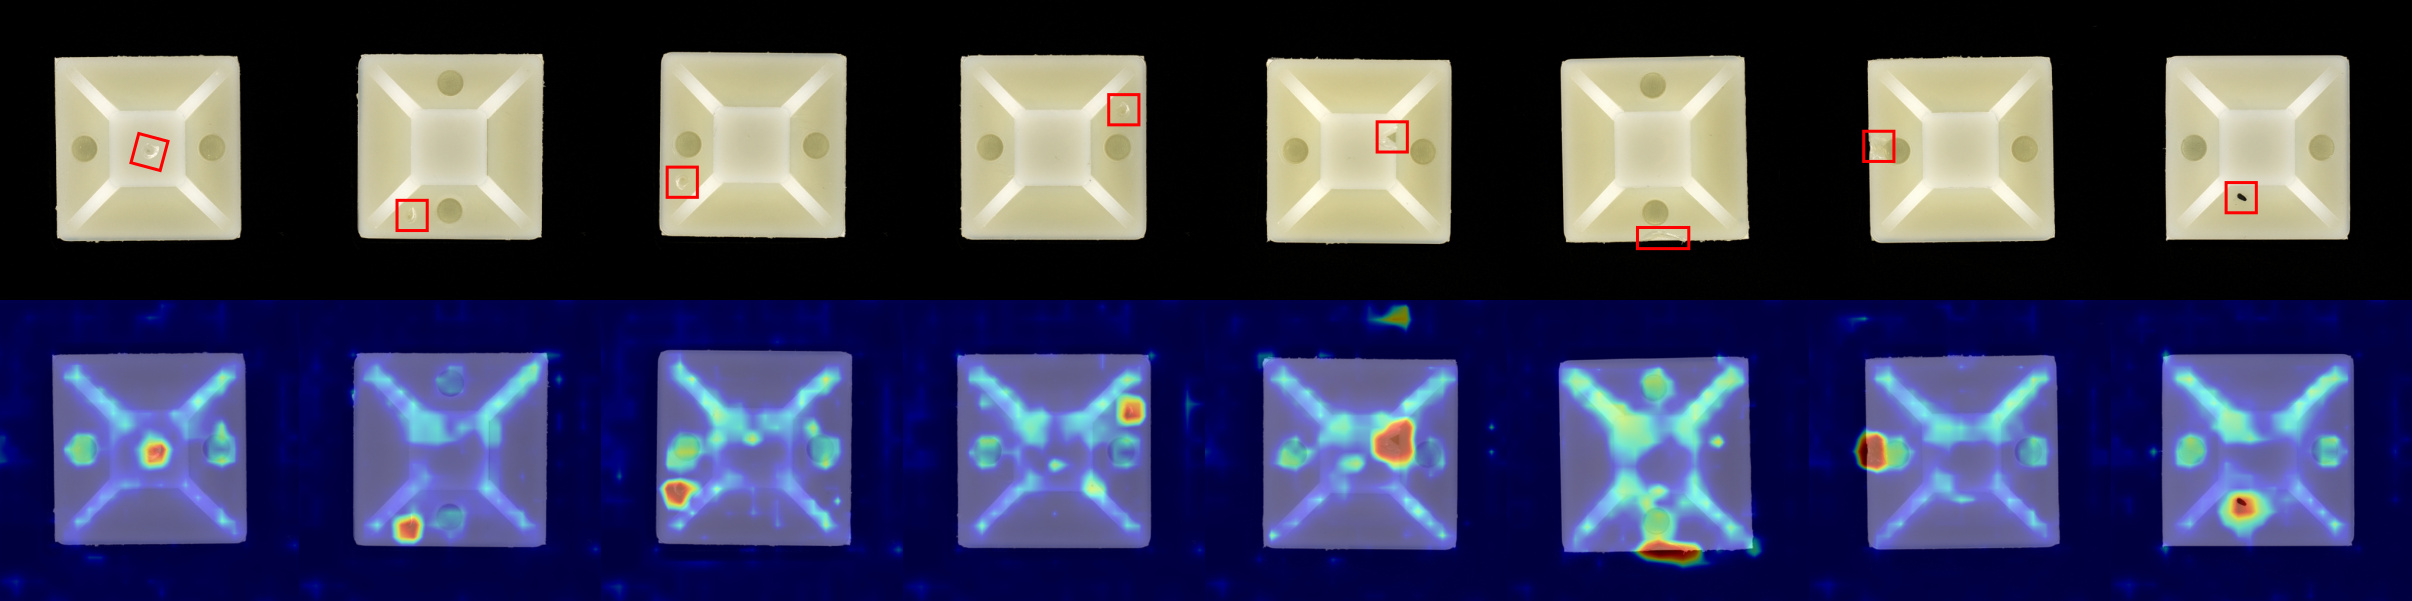
\includegraphics[width=\textwidth]{imgs/rolled_strip_base.jpg}
  \caption{This visualization showcases the rolled strip base product from the Real-IAD dataset. The first row represents the input with the anomaly highlighted. The second row presents the segmentation results
from our model.}
   \label{fig:rolled_strip_base}
\end{figure*}

\begin{figure*}
  \centering
  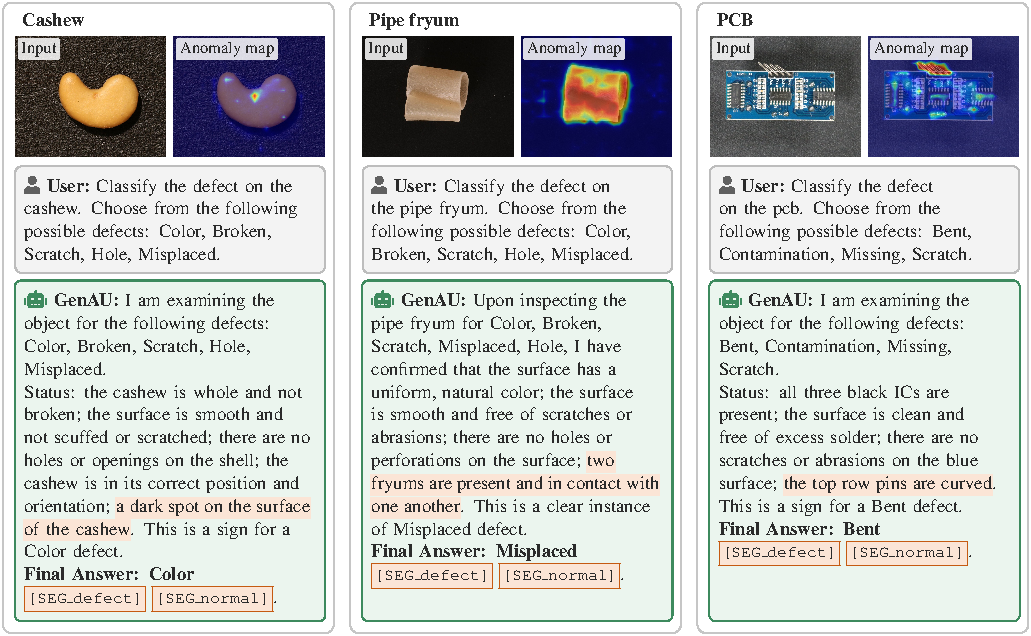
\includegraphics[width=\textwidth]{imgs/GenAU_Dialogue.pdf}
  \caption{This visualization showcases the abilities of GenAU. Given the input prompt and the image, the model reasons over the possible defects, identifies the correct one and outputs a segmentation mask.}
   \label{fig:text}
\end{figure*}



\end{document}
